\documentclass{article}
%%%%%%%%%%%%%%%%%%%%%%%%%%%%%%%%%%%%%%%%%%%%%%%%%%%%%%%%%%%%%%%%%%%%%%%%%%%%%%%%%%%%%%%%%%%%%%%%%%%%%%%%%%%%%%%%%%%%%%%%%%%%%%%%%%%%%%%%%%%%%%%%%%%%%%%%%%%%%%%%%%%%%%%%%%%%%%%%%%%%%%%%%%%%%%%%%%%%%%%%%%%%%%%%%%%%%%%%%%%%%%%%%%%%%%%%%%%%%%%%%%%%%%%%%%%%
\usepackage{eurosym}
\usepackage[top=1cm,bottom=2cm,left=1.5cm,right=1.5cm,a4paper]{geometry}
\usepackage{amsmath,amssymb,mathrsfs}
\usepackage{amsthm}
\usepackage[colorlinks]{hyperref}
%\usepackage[nameinlink]{cleveref}
\usepackage{url}
\usepackage{graphicx,color,epsfig}
\usepackage{epstopdf}
\usepackage{amsfonts}
\usepackage{caption}
\usepackage{enumerate}
\usepackage{enumitem}
\usepackage{float}
\usepackage{booktabs}
\usepackage{graphicx}
\usepackage{subcaption}
\usepackage{array}
\usepackage{booktabs}
\usepackage{fancyhdr}
\usepackage{eurosym}
\usepackage{cite}
\usepackage{cleveref}
\usepackage{upgreek}
\usepackage{enumitem}
\usepackage{xcolor,rotating}
\usepackage{placeins}
\usepackage{color,soul}
\setcounter{MaxMatrixCols}{10}
%TCIDATA{OutputFilter=Latex.dll}
%TCIDATA{Version=5.50.0.2953}
%TCIDATA{<META NAME="SaveForMode" CONTENT="1">}
%TCIDATA{BibliographyScheme=Manual}
%TCIDATA{LastRevised=Thursday, April 25, 2019 13:23:17}
%TCIDATA{<META NAME="GraphicsSave" CONTENT="32">}
%\renewcommand{\tablename}{{\small F}\scriptsize{IGURE}}
\DeclareMathOperator{\sech}{sech}
\DeclareMathOperator{\csch}{csch}
\newtheorem{theorem}{Theorem}
\newtheorem{acknowledgement}[theorem]{Acknowledgement}
\newtheorem{conclusion}[theorem]{Conclusion}
\newtheorem{condition}[theorem]{Condition}
\newtheorem{corollary}[theorem]{Corollary}
\newtheorem{definition}[theorem]{Definition}
\newtheorem{lemma}[theorem]{Lemma}
\newtheorem{proposition}[theorem]{Proposition}
\newtheorem{remark}[theorem]{Remark}
%\newenvironment{proof}[1][Proof]{\noindent\textbf{#1.} }{\ \rule{0.5em}{0.5em}}
\usepackage[symbol]{footmisc}
\def\correspondingauthor{\footnote{Corresponding author.}}
\numberwithin{equation}{section}
\newlist{steps}{enumerate}{1}
\setlist[steps, 1]{label = Step \arabic*:}
\usepackage{multicol}
\hypersetup{pdftitle={},% title
    pdfauthor={Lanre Akinyemi},     % author
    %pdfsubject={Differential Equations},   % subject of the document
    pdfcreator={pdftex},   % creator of the document
    pdfproducer={Texmaker}, % producer of the document
    pdfkeywords={}, % list of keywords
    colorlinks=true,       % false: boxed links; true: colored links
    linkcolor=blue,          % color of internal links
    citecolor=blue,        % color of links to bibliography
    filecolor=magenta,      % color of file links
    urlcolor=blue           % color of external links
}
\setcounter{MaxMatrixCols}{10}
%%%%%%%%%%%%%%%%%%%%%%%%%%%%%%%%%%%%
\newcommand{\capu}{\mathcal{D}}
%%%%%%%%%%%%%%%%%%%%%%%%%%%%%%%%%%%%
\renewcommand{\equationautorefname}{Eq.}
\Crefname{figure}{Fig.}{Figs.}
\Crefname{table}{Tab.}{Tabs.}
\makeatletter
\let\oldtheequation\theequation
\renewcommand\tagform@[1]{\maketag@@@{\ignorespaces#1\unskip\@@italiccorr}}
\renewcommand\theequation{(\oldtheequation)}
\makeatother
%%%%%%%%%%%%%%%%%%%%%%%%%%%%%%%%%%%
%\newtheorem{theorem}{Theorem}[section]
\newtheorem{case}{Case}
%\newtheorem{definition}[theorem]{Definition}
%\newtheorem{example}[theorem]{Example}
%\newtheorem{lemma}[theorem]{Lemma}
%\newtheorem{remark}[theorem]{Remark}
%\newenvironment{proof}[1][Proof]{\noindent\textbf{#1.} }{\ \rule{0.5em}{0.5em}}
\usepackage[symbol]{footmisc}
\renewcommand{\baselinestretch}{1.2}
%%%%%%%%%%%%%%%%%%%%%%%%%%%%%%%%%%%%
\date{}
%opening\def\correspondingauthor{\footnote{Corresponding author.}}
\begin{document}
\title{ \textbf{Exact soliton solution for $(3+1)$-dimensional Kortwege-de-Vries-Zakharov-Kuznetzov equation along with bifurcation analysis  }}
\author{ Ali Akg\"{u}l$^{1,2,*}$, Romana Ashraf $^{3}$, Farrah Ashraf $^{3}$, Rehan Khursheed $^{4}$,  \\
$^{1}$ Department of Electronics and Communication Engineering,\\ Saveetha School of Engineering,
SIMATS, Chennai, Tamilnadu, India.\\
$^{2}$ Siirt University, Art and Science Faculty, Department of Mathematics, 56100 Siirt, Türkiye.\\
$^{3}$ Department of Computer Science $ \& $ IT,\\ The University of Lahore, Lahore, Pakistan.\\
$^{4}$ Department of Mathematics and Statistics,\\ The University of Lahore, Lahore, Pakistan.\\
Corresponding (*): aliakgul00727@gmail.com\\
e-mail: \{dr.romanauetian, f.as70000, rehankhursheed468 \}@gmail.com }
\date{ }
\maketitle
% !TeX spellcheck = en_US
\begin{abstract}
\noindent
This paper offers an in-depth analytical and dynamical study of the $(3+1)$-dimensional Korteweg-de-Vries-Zakharov-Kuznetsov (KdV-ZK) equation, which plays an important role in plasma physics and non-linear wave phenomena. By applying the unified method, several classes of exact traveling-wave soliton solutions are obtained in a systematic manner, including kink-type, singular and periodic structures. The analysis begins with a traveling-wave transformation that reduces the governing partial differential equation to an ordinary differential equation, which is then solved using a generalized trial function together with Riccati-type auxiliary equations. A qualitative bifurcation analysis of the related planar dynamical system is carried out in conjunction with the analytical derivation. This analysis looks at phase portraits across different parameter settings and finds equilibrium spots. Numerous dynamical aspects are shown in the results, including homoclinic, heteroclinic and periodic trajectories, which represent solitary waves, kink and anti-kink solutions and periodic wave patterns, respectively. To illustrate the spatial and temporal features of the representative solutions, visual charts are shown. Overall, the study improves knowledge of the interplay between dispersion and non-linearity in higher dimensions non-linear wave systems and broadens the range of exact solutions accessible for the (3+1)-dimensional KdV-ZK equation.\\
\textbf{Key words}:Unified approach method, Exact soliton solutions, Kortwege-de-Vries-Zakharov-Kuznetzov equation, Kink shaped soliton, Singular soliton and Periodic soliton solutions.
\end{abstract}
\section{Introduction}
\noindent Analytical solutions of non-linear partial differential equations (NLPDEs) play a crucial role in the theory of non-linear phenomena. Such equations arise in many natural processes and appear across a wide range of scientific and applied disciplines, including mathematical physics, fluid mechanics and hydrodynamics. Numerous fields, including optics, birefringent fiber systems, elastic media, chemical processes, cosmology, ecology, quantum mechanics, geology, plasma physics, wave propagation and shallow water dynamics, use NLPDEs extensively to describe and evaluate phenomena. \cite{b1,b2,b3,b4,b5,b6,b7,b8,b9,b10,b11,b12}. Since exact soliton solutions offer clear insights into the non-linear dynamics and stability of solitary waves. These solutions act as standards for numerical simulations and approximate analytical techniques in addition to illuminating the process of energy localization and transport in non-linear media. The significance and structure of NLPDEs led to a growth in their applications throughout time. Mean-while, several new constructive techniques have been developed and changed throughout time such as sine-cosine method \cite{b13,b14}, Riccati-Bernoulli sub-ODE method \cite{b15}, Optimal homotopy asymptotic method \cite{b16,b17,b18,b19}, Method of Homotopy perturbation \cite{b20}, Method of variational iteration \cite{b21}, Method of The ($\frac{G'}{G}$)-Expansion \cite{b22,b23,b24}, The method of Exp-Function \cite{b25,b26,b27,b28}, Method of Modified simple equation \cite{b29,b30}, Method of tanh function \cite{b31,b32,b33}, Method of Kudryashov \cite{b34,b35}, Method of The Trial equation \cite{b36}, Method of the Backscatter \cite{b37}, B\"{a}cklund transform\cite{b38}, Method of Hirota bilinear \cite{b39}, Homogeneous balance method\cite{b40} and Method of Jacobi and Weierstrass elliptic function \cite{b41} etc.\\
Bifurcation analysis of the traveling-wave system related to the KdV-ZK equation offers a better comprehension of the qualitative dynamics than the production of exact solutions. Bifurcation theory makes it possible to categorize wave patterns according to equilibrium points and their stability in the relevant dynamical system, including kink-type solutions, periodic waves and solitary waves. This combined viewpoint provides a thorough framework for examining the complex interplay between dispersion and non-linearity in multidimensional wave propagation by combining bifurcation analysis with the building of exact solutions. With a focus on obtaining precise soliton solutions of the (3+1)-dimensional KdV-ZK equation, this study presents a thorough bifurcation analysis of the related reduced dynamical system. The obtained results give significant physical explanations of wave shapes found in plasma and other comparable nonlinear media, while also expanding the model's solution space.\\
This study uses an effective method to produce a range of soliton solutions for (3 + 1)-dimensional KdV-ZK, which is simulated for plasma physics \cite{b42,b43}. It is provided as
\begin{eqnarray}\label{KDVZK}
u_{t}+a u^2 u_{x}+b u_{xxx}+d(u_{yy}-u_{zz})_{x}=0,
\end{eqnarray}
where \emph{u} is the wave profile, \emph{x} and \emph{t} are the scaled spatial and temporal variables respectively. An appropriate transformation most frequently a traveling-wave transformation is typically applied to translate a Partial Differential Equation (PDE) into an Ordinary Differential Equation (ODE). By integrating them into a single new variable commonly referred to as the wave variable, the goal is to decrease the number of independent variables. This method assumes that the solution takes the shape of a moving wave and is dependent on both space and time factors.
\section{Unified Approach Methodology }
The methodology of unified approach method has the following steps
\subsection{Various Steps in the Unified Approach Technique}
\textbf{Step 1:}
We employ a traveling-wave transformation to convert the governing partial differential equation into an ordinary differential equation.
\begin{eqnarray}\label{PDE}
\Omega(u_x,u_t,u_{xt},u_{xx},u_{xxx}........)=0,
\end{eqnarray}
into ODE form (By combining the variables we get)
\begin{eqnarray}\label{ODE}
\Pi(U',U'',U''',.............)=0.
\end{eqnarray}\\\
\textbf{Step 2:}
Assuming solution to solve the problem
\begin{eqnarray}\label{TF}
\frac{d}{d \zeta}\eta \! \left(\zeta \right) =H_{0}+ \sum_{j=1}^M H_{j}\eta \left(\zeta \right)^{j}+\sum_{j=1}^M \frac{F_{j}}{\eta \left(\zeta \right)^{j}}.
\end{eqnarray}
\textbf{Step 3:}
Calculate the value of M by balancing the highest order derivative term with the highest order non-linear term involved in the ODE form of the problem.\\
Reccati Equation of the form
\begin{eqnarray}\label{RE}
\frac{d}{d \zeta}\eta \! \left(\zeta \right) =\eta \! \left(\zeta \right)^{2}+N.
\end{eqnarray}
Here we have different families ${\eta(\zeta)}$ of Eq. \ref{RE} depending upon the value of \emph{N} (The value of \emph{N} can be Zero, negative and positive).\\
\textbf{when $\textbf{ N $<$ 0} $ }
\begin{align}\label{FAM1}
\begin{cases}\\
\textbf{(i)}\quad \eta \! \left(\zeta \right) =\frac{-\sqrt{-\left(K^{2}+L^{2}\right) N}-K \sqrt{-N}\, \cosh \, \left(2 \sqrt{-N}\, \left(x+y+z-ct +\psi \right)\right)}{K \sinh \, \left(2 \sqrt{-N}\, \left(x+y+z-ct +\psi \right)\right)+L},\\
\textbf{(ii)}\quad \eta \! \left(\zeta \right) =\frac{\sqrt{-\left(K^{2}+L^{2}\right) N}-K \sqrt{-N}\, \cosh \, \left(2 \sqrt{-N}\, \left(x+y+z-ct +\psi \right)\right)}{K \sinh \, \left(2 \sqrt{-N}\, \left(x+y+z-ct +\psi \right)\right)+L},\\
\textbf{(iii)}\quad \eta \! \left(\zeta \right) =-\sqrt{-N}+\frac{2 K \sqrt{-N}}{K +\cosh \, \left(2 \sqrt{-N}\, \left(x+y+z-ct +\psi \right)\right)-\sinh \, \left(2 \sqrt{-N}\, \left(x+y+z-ct +\psi \right)\right)},\\
\textbf{(iv)}\quad \eta \! \left(\zeta \right) =\sqrt{-N}+\frac{2 K \sqrt{-N}}{K +\cosh \, \left(2 \sqrt{-N}\, \left(x+y+z-ct +\psi \right)\right)-\sinh \, \left(2 \sqrt{-N}\, \left(x+y+z-ct +\psi \right)\right)}.\\
\end{cases}
\end{align}
\textbf{when $\textbf{ N $>$ 0} $ }
\noindent
\begin{align}\label{FAM2}
\begin{cases}\\
\textbf{(i)}\quad \eta \! \left(\zeta \right) =\frac{-\sqrt{\left(K^{2}+L^{2}\right) N}-K \sqrt{N}\, \cos \, \left(2 \sqrt{N}\, \left(x+y+z-ct +\psi \right)\right)}{K \sin \, \left(2 \sqrt{N}\, \left(x+y+z-ct +\psi \right)\right)+L},\\\
\textbf{(ii)}\quad \eta \! \left(\zeta \right) =\frac{\sqrt{\left(K^{2}+L^{2}\right) N}-K \sqrt{N}\, \cos \, \left(2 \sqrt{N}\, \left(x+y+z-ct +\psi \right)\right)}{K \sin \, \left(2 \sqrt{N}\, \left(x+y+z-ct +\psi \right)\right)+L},\\\
\textbf{(iii)}\quad \eta \! \left(\zeta \right) =-i \sqrt{N}+\frac{2 i K \sqrt{N}}{K +\cos \, \left(2 \sqrt{N}\, \left(x+y+z-ct +\psi \right)\right)-i \sin \, \left(2 \sqrt{N}\, \left(x+y+z-ct +\psi \right)\right)},\\\
\textbf{(iv)}\quad \eta \! \left(\zeta \right) =i \sqrt{N}+\frac{2 i K \sqrt{N}}{K +\cos \, \left(2 \sqrt{N}\, \left(x+y+z-ct +\psi \right)\right)-i \sin \, \left(2 \sqrt{N}\, \left(x+y+z-ct +\psi \right)\right)}.\\\
\end{cases}
\end{align}
\textbf{when $\textbf{ N $=$ 0}$ }
\begin{eqnarray}\label{FAM3}
\quad \eta \! \left(\zeta \right) = -\frac{1}{x+y+z-ct +\psi}.
\end{eqnarray}
\section{Solution of Kortwege-de-Vries-Zakharov-Kuznetzov Equation}

Non-linear KdV-ZK equation of the form
\begin{eqnarray}\label{PDE1}
u_{t}+a u^2 u_{x}+b u_{xxx}+d(u_{yy}-u_{zz})_{x}=0,
\end{eqnarray}
The traveling wave transformation is
\begin{eqnarray}\label{TF1}
u(x,y,z,t)=U(\zeta), \qquad \zeta=x+y+z-ct,
\end{eqnarray}
By using the transformation Eq. \ref{TF1} in  Eq. \ref{PDE1} we get
\begin{eqnarray}
    -c\,U'+\kappa U^2 U'+ \mu U'''+2\upsilon U'''=0,
\end{eqnarray}
Integrating the result twice we get our required ODE form of KdV-ZK equation
\begin{eqnarray}\label{ODE1}
    -c\,U+\kappa \frac{U^3}{3}+ (\mu+2\upsilon)U''=0,
\end{eqnarray}
where $\kappa$, $\upsilon$ and $\mu$ are arbitrary parameters.\\
We obtained \emph{M} = 1 by applying the Homogeneous Balancing Principle (which involves balancing the maximum degree non-linear term $U^{2}$ with the maximum order derivative term $U''$) in Eq. \ref{ODE1} \\
Now by replacing $M$ = 1 in equation in Eq. \ref{TF} we get
\begin{eqnarray}\label{S}
U  \left(\zeta \right) =H_{0}+H_{1} \eta \left(\zeta \right)+\frac{F_{1}}{\eta \left(\zeta \right)}.
\end{eqnarray}
here we need to find the constants involved in $U{(\zeta)}$ which are $H_{0}$, $H_{1}$, $H_{2}$, $F_{1}$ and $F_{2}$,
The $\eta{(\zeta)}$ represents (the families given) the solutions of Eq. \ref{RE}.\\
Now substitute Eq. \ref{RE} and Eq. \ref{S} in Eq. \ref{ODE1} then simplify resulting equation to get the coefficients of all powers of ${\eta(\zeta)}$ and set all the coefficients of the various powers of $\eta{(\zeta)}$ to zero to produce a set of simultaneous solvable algebraic equations.
The coefficients of different powers of $\eta{(\zeta)}$ are as follows\\
\begin{align}
\begin{cases}
\eta{(\zeta)}^{-3} :\;\,\quad 4 \left(-\frac{F_{1}^{2} \alpha}{12}+N^{2} \left(\frac{\beta}{2}+\nu \right)\right) F_{1} = 0, \\
\eta{(\zeta)}^{-2} :\;\,\quad -\alpha  H_{0} F_{1}^{2} = 0,\\
\eta{(\zeta)}^{-1} :\,\;\quad 4 \left(-\frac{\alpha  F_{1} H_{1}}{4}-\frac{\alpha  H_{0}^{2}}{4}+\left(\frac{\beta}{2}+\nu \right) N -\frac{c}{4}\right) F_{1} = 0,\\
\eta{(\zeta)}^{0}  :\qquad -H_{0} \left(\frac{1}{3} \alpha  H_{0}^{2}+2 \alpha  F_{1} H_{1}+c \right) = 0,\\
\eta{(\zeta)}^{1}  :\qquad 4 H_{1} \left(-\frac{\alpha  F_{1} H_{1}}{4}-\frac{\alpha  H_{0}^{2}}{4}+\left(\frac{\beta}{2}+\nu \right) N -\frac{c}{4}\right) = 0,\\
\eta{(\zeta)}^{2}  :\qquad -\alpha  H_{0} H_{1}^{2} = 0, \\
\eta{(\zeta)}^{3}  :\qquad 4 H_{1} \left(-\frac{\alpha  H_{1}^{2}}{12}+\nu +\frac{\beta}{2}\right) = 0.\\
\end{cases}
\end{align}
Now by using Mathematica software we find the simultaneous solution sets of these equations.\\\
\textbf{Set I:}
\begin{eqnarray}\label{set1}
c = 2N(\beta+2v),\quad\,F_{1} = 0,\quad\, H_{0} = 0\quad\,{\&}\quad\,H_{1} = \frac{\sqrt{6}\sqrt{\beta+2v}}{\sqrt{\alpha}}.
\end{eqnarray}
\begin{equation}\label{U1}
    U_{1}\! \left(\zeta \right) =
\frac{\left(-\sqrt{-\left(K^{2}+L^{2}\right) N}-K \sqrt{-N}\, \cosh \! \left(2 \sqrt{-N}\, \left(x + y + z  -2 N \left(\beta +2 v \right) t +\phi \right)\right)\right) \sqrt{6}\, \sqrt{\beta +2 v}}{\left(K \sinh \! \left(2 \sqrt{-N}\, \left(x + y + z -2 N \left(\beta +2 v \right) t +\phi \right)\right)+L \right) \sqrt{\alpha}},
\end{equation}
\begin{equation}\label{U2}
    U_{2}\! \left(\zeta \right) =
\frac{\left(\sqrt{-\left(K^{2}+L^{2}\right) N}-K \sqrt{-N}\, \cosh \! \left(2 \sqrt{-N}\, \left(x + y + z  -2 N \left(\beta +2 v \right) t +\phi \right)\right)\right) \sqrt{6}\, \sqrt{\beta +2 v}}{\left(K \sinh \! \left(2 \sqrt{-N}\, \left(x + y + z  -2 N \left(\beta +2 v \right) t +\phi \right)\right)+L \right) \sqrt{\alpha}},
\end{equation}
\begin{equation}\label{U3}
    U_{3}\! \left(\zeta \right) =
\frac{\left(\sqrt{-N}+\frac{2 K \sqrt{-N}}{K +\cosh \left(2 \sqrt{-N}\, \left(x + y + z  -2 N \left(\beta +2 v \right) t +\phi \right)\right)-\sinh \left(2 \sqrt{-N}\, \left(x + y + z  -2 N \left(\beta +2 v \right) t +\phi \right)\right)}\right) \sqrt{6}\, \sqrt{\beta +2 v}}{\sqrt{\alpha}},
\end{equation}
\begin{equation}\label{U4}
    U_{4}\! \left(\zeta \right) =
\frac{\left(-\sqrt{-N}+\frac{2 K \sqrt{-N}}{K +\cosh \left(2 \sqrt{-N}\, \left(x + y + z  -2 N \left(\beta +2 v \right) t +\phi \right)\right)-\sinh \left(2 \sqrt{-N}\, \left(x + y + z  -2 N \left(\beta +2 v \right) t +\phi \right)\right)}\right) \sqrt{6}\, \sqrt{\beta +2 v}}{\sqrt{\alpha}},
\end{equation}
\begin{equation}\label{U5}
    U_{5} \! \left(\zeta \right) =
\frac{\sqrt{6}\, \sqrt{\beta +2 v}\, \left(\sqrt{\left(K^{2}+L^{2}\right) N}-K \sqrt{N}\, \cos \! \left(2 \sqrt{N}\, \left(x -2 N \left(\beta +2 v \right) t +\phi +y +z \right)\right)\right)}{\sqrt{\alpha}\, \left(K \sin \! \left(2 \sqrt{N}\, \left(x -2 N \left(\beta +2 v \right) t +\phi +y +z \right)\right)+L \right)},
\end{equation}
\begin{equation}\label{U6}
    U_{6} \! \left(\zeta \right) =
\frac{\sqrt{6}\, \sqrt{\beta +2 v}\, \left(-\sqrt{\left(K^{2}+L^{2}\right) N}-K \sqrt{N}\, \cos \! \left(2 \sqrt{N}\, \left(x -2 N \left(\beta +2 v \right) t +\phi +y +z \right)\right)\right)}{\sqrt{\alpha}\, \left(K \sin \! \left(2 \sqrt{N}\, \left(x -2 N \left(\beta +2 v \right) t +\phi +y +z \right)\right)+L \right)},
\end{equation}
\begin{equation}\label{U7}
    U_{7} \! \left(\zeta \right) =
\frac{\sqrt{6}\, \sqrt{\beta +2 v}\, \left(i \sqrt{N}+\frac{2 i K \sqrt{N}}{K +\cos \left(2 \sqrt{N}\, \left(x +y +z -2 N \left(\beta +2 v \right) t +\phi \right)\right)-i \sin \left(2 \sqrt{N}\, \left(x +y +z -2 N \left(\beta +2 v \right) t +\phi \right)\right)}\right)}{\sqrt{\alpha}},
\end{equation}
\begin{equation}\label{U8}
    U_{8} \! \left(\zeta \right) =
\frac{\sqrt{6}\, \sqrt{\beta +2 v}\, \left(-i \sqrt{N}+\frac{2 i K \sqrt{N}}{K +\cos \left(2 \sqrt{N}\, \left(x +y +z -2 N \left(\beta +2 v \right) t +\phi \right)\right)-i \sin \left(2 \sqrt{N}\, \left(x +y +z -2 N \left(\beta +2 v \right) t +\phi \right)\right)}\right)}{\sqrt{\alpha}},
\end{equation}
\begin{equation}\label{U9}
    U_{9} \! \left(\zeta \right) =
-\frac{\sqrt{6}\, \sqrt{\beta +2 v}}{\sqrt{\alpha}\, \left(x -2 N \left(\beta +2 v \right) t +\phi +y +z \right)}.
\end{equation}
\textbf{Set II:}
\begin{eqnarray}\label{set2}
c = -4N(\beta+2v),\quad\,F_{1} = \frac{\sqrt{6}N\sqrt{\beta+2v}}{\sqrt{\alpha}}.,\quad\, H_{0} = 0\quad\,{\&}\quad\,H_{1} = \frac{\sqrt{6}\sqrt{\beta+2v}}{\sqrt{\alpha}}.
\end{eqnarray}
\begin{equation}\label{U10}
    U_{10}\! \left(\zeta \right) =
\frac{\sqrt{6}\, \sqrt{\beta +2 v}\, \left(-\sqrt{-\left(K^{2}+L^{2}\right) N}-K \sqrt{-N}\, \cosh \! \left(2 \sqrt{-N}\, \left(x +y +z -4 N \left(\beta +2 v \right) t +\phi \right)\right)\right)}{\sqrt{\alpha}\, \left(K \sinh \! \left(2 \sqrt{-N}\, \left(x +y +z -4 N \left(\beta +2 v \right) t +\phi \right)\right)+L \right)}+\nonumber
\end{equation}
\begin{eqnarray}
\frac{\sqrt{6}\, N \sqrt{\beta +2 v}\, \left(K \sinh \! \left(2 \sqrt{-N}\, \left(x +y +z -4 N \left(\beta +2 v \right) t +\phi \right)\right)+L \right)}{\sqrt{\alpha}\, \left(-\sqrt{-\left(K^{2}+L^{2}\right) N}-K \sqrt{-N}\, \cosh \! \left(2 \sqrt{-N}\, \left(x +y +z -4 N \left(\beta +2 v \right) t +\phi \right)\right)\right)},
\end{eqnarray}
\begin{equation}\label{U11}
    U_{11}\! \left(\zeta \right) =
\frac{\sqrt{6}\, \sqrt{\beta +2 v}\, \left(\sqrt{-\left(K^{2}+L^{2}\right) N}-K \sqrt{-N}\, \cosh \! \left(2 \sqrt{-N}\, \left(x +y +z -4 N \left(\beta +2 v \right) t +\phi \right)\right)\right)}{\sqrt{\alpha}\, \left(K \sinh \! \left(2 \sqrt{-N}\, \left(x +y +z -4 N \left(\beta +2 v \right) t +\phi \right)\right)+L \right)}+\nonumber
\end{equation}
\begin{equation}
\frac{\sqrt{6}\, N \sqrt{\beta +2 v}\, \left(K \sinh \! \left(2 \sqrt{-N}\, \left(x +y +z -4 N \left(\beta +2 v \right) t +\phi \right)\right)+L \right)}{\sqrt{\alpha}\, \left(\sqrt{-\left(K^{2}+L^{2}\right) N}-K \sqrt{-N}\, \cosh \! \left(2 \sqrt{-N}\, \left(x +y +z -4 N \left(\beta +2 v \right) t +\phi \right)\right)\right)},
\end{equation}
\begin{equation}\label{U12}
    U_{12}\! \left(\zeta \right) =
\frac{\sqrt{6}\, \sqrt{\beta +2 v}\, \left(\sqrt{-N}+\frac{2 K \sqrt{-N}}{K +\cosh \left(2 \sqrt{-N}\, \left(x +y +z -4 N \left(\beta +2 v \right) t +\phi \right)\right)-\sinh \left(2 \sqrt{-N}\, \left(x +y +z -4 N \left(\beta +2 v \right) t +\phi \right)\right)}\right)}{\sqrt{\alpha}}+\nonumber
\end{equation}
\begin{equation}\frac{\sqrt{6}\, N \sqrt{\beta +2 v}}{\sqrt{\alpha}\, \left(\sqrt{-N}+\frac{2 K \sqrt{-N}}{K +\cosh \left(2 \sqrt{-N}\, \left(x +y +z -4 N \left(\beta +2 v \right) t +\phi \right)\right)-\sinh \left(2 \sqrt{-N}\, \left(x +y +z -4 N \left(\beta +2 v \right) t +\phi \right)\right)}\right)},
\end{equation}
\begin{equation}\label{U13}
    U_{13}\! \left(\zeta \right) =
\frac{\sqrt{6}\, \sqrt{\beta +2 v}\, \left(-\sqrt{-N}+\frac{2 K \sqrt{-N}}{K +\cosh \left(2 \sqrt{-N}\, \left(x +y +z -4 N \left(\beta +2 v \right) t +\phi \right)\right)-\sinh \left(2 \sqrt{-N}\, \left(x +y +z -4 N \left(\beta +2 v \right) t +\phi \right)\right)}\right)}{\sqrt{\alpha}}+\nonumber
\end{equation}
\begin{equation}
\frac{\sqrt{6}\, N \sqrt{\beta +2 v}}{\sqrt{\alpha}\, \left(-\sqrt{-N}+\frac{2 K \sqrt{-N}}{K +\cosh \left(2 \sqrt{-N}\, \left(x +y +z -4 N \left(\beta +2 v \right) t +\phi \right)\right)-\sinh \left(2 \sqrt{-N}\, \left(x +y +z -4 N \left(\beta +2 v \right) t +\phi \right)\right)}\right)},
\end{equation}
\begin{equation}\label{U14}
    U_{14}\! \left(\zeta \right) =
\frac{\sqrt{6}\, \sqrt{\beta +2 v}\, \left(\sqrt{\left(K^{2}+L^{2}\right) N}-K \sqrt{N}\, \cos \! \left(2 \sqrt{N}\, \left(-4 N \left(\beta +2 v \right) t +\phi +x +y +z \right)\right)\right)}{\sqrt{\alpha}\, \left(K \sin \! \left(2 \sqrt{N}\, \left(-4 N \left(\beta +2 v \right) t +\phi +x +y +z \right)\right)+L \right)}+\nonumber
\end{equation}
\begin{equation}
\frac{\sqrt{6}\, N \sqrt{\beta +2 v}\, \left(K \sin \! \left(2 \sqrt{N}\, \left(-4 N \left(\beta +2 v \right) t +\phi +x +y +z \right)\right)+L \right)}{\sqrt{\alpha}\, \left(\sqrt{\left(K^{2}+L^{2}\right) N}-K \sqrt{N}\, \cos \! \left(2 \sqrt{N}\, \left(-4 N \left(\beta +2 v \right) t +\phi +x +y +z \right)\right)\right)},
\end{equation}
\begin{equation}\label{U15}
    U_{15}\! \left(\zeta \right) =
\frac{\sqrt{6}\, \sqrt{\beta +2 v}\, \left(-\sqrt{\left(K^{2}+L^{2}\right) N}-K \sqrt{N}\, \cos \! \left(2 \sqrt{N}\, \left(-4 N \left(\beta +2 v \right) t +\phi +x +y +z \right)\right)\right)}{\sqrt{\alpha}\, \left(K \sin \! \left(2 \sqrt{N}\, \left(-4 N \left(\beta +2 v \right) t +\phi +x +y +z \right)\right)+L \right)}+\nonumber
\end{equation}
\begin{equation}
\frac{\sqrt{6}\, N \sqrt{\beta +2 v}\, \left(K \sin \! \left(2 \sqrt{N}\, \left(-4 N \left(\beta +2 v \right) t +\phi +x +y +z \right)\right)+L \right)}{\sqrt{\alpha}\, \left(\sqrt{-\left(K^{2}+L^{2}\right) N}-K \sqrt{N}\, \cos \! \left(2 \sqrt{N}\, \left(-4 N \left(\beta +2 v \right) t +\phi +x +y +z \right)\right)\right)},
\end{equation}
\begin{equation}\label{U16}
    U_{16}\! \left(\zeta \right) =
\frac{\sqrt{6}\, \sqrt{\beta +2 v}\, \left(i \sqrt{N}+\frac{2 i K \sqrt{N}}{K +\cos \left(2 \sqrt{N}\, \left(-4 N \left(\beta +2 v \right) t +\phi +x +y +z \right)\right)-i \sin \left(2 \sqrt{N}\, \left(-4 N \left(\beta +2 v \right) t +\phi +x +y +z \right)\right)}\right)}{\sqrt{\alpha}}+\nonumber
\end{equation}
\begin{equation}
\frac{\sqrt{6}\, N \sqrt{\beta +2 v}}{\sqrt{\alpha}\, \left(i \sqrt{N}+\frac{2 i K \sqrt{N}}{K +\cos \left(2 \sqrt{N}\, \left(-4 N \left(\beta +2 v \right) t +\phi +x +y +z \right)\right)-i \sin \left(2 \sqrt{N}\, \left(-4 N \left(\beta +2 v \right) t +\phi +x +y +z \right)\right)}\right)},
\end{equation}
\begin{equation}\label{U17}
    U_{17}\! \left(\zeta \right) =
\frac{\sqrt{6}\, \sqrt{\beta +2 v}\, \left(-i \sqrt{N}+\frac{2 i K \sqrt{N}}{K +\cos \left(2 \sqrt{N}\, \left(-4 N \left(\beta +2 v \right) t +\phi +x +y +z \right)\right)-i \sin \left(2 \sqrt{N}\, \left(-4 N \left(\beta +2 v \right) t +\phi +x +y +z \right)\right)}\right)}{\sqrt{\alpha}}+\nonumber
\end{equation}
\begin{equation}
\frac{\sqrt{6}\, N \sqrt{\beta +2 v}}{\sqrt{\alpha}\, \left(-i \sqrt{N}+\frac{2 i K \sqrt{N}}{K +\cos \left(2 \sqrt{N}\, \left(-4 N \left(\beta +2 v \right) t +\phi +x +y +z \right)\right)-i \sin \left(2 \sqrt{N}\, \left(-4 N \left(\beta +2 v \right) t +\phi +x +y +z \right)\right)}\right)},
\end{equation}
\begin{equation}\label{U18}
    U_{18}\! \left(\zeta \right) =
-\frac{\sqrt{6}\, \sqrt{\beta +2 v}}{\sqrt{\alpha}\, \left(-4 N \left(\beta +2 v \right) t +\phi +x +y +z \right)}+\frac{\sqrt{6}\, N \sqrt{\beta +2 v}\, \left(4 N \left(\beta +2 v \right) t -\phi -x -y -z \right)}{\sqrt{\alpha}}.
\end{equation}
\textbf{Set III:}
\begin{eqnarray}\label{set3}
c = 2N(\beta+2v),\quad\,F_{1} = \frac{\sqrt{6} N \sqrt{\beta+2v}}{\sqrt{\alpha}},\quad\, H_{0} = 0\quad\,{\&}\quad\,H_{1} = 0.
\end{eqnarray}
\begin{equation}\label{U19}
    U_{19} \! \left(\zeta \right) =
\frac{\sqrt{6}\, \sqrt{\beta +2 v}\, N \left(K \sinh \! \left(2 \sqrt{-N}\, \left(x +y +z -2 N \left(\beta +2 v \right) t +\phi \right)\right)+L \right)}{\sqrt{\alpha}\, \left(-\sqrt{-\left(K^{2}+L^{2}\right) N}-K \sqrt{-N}\, \cosh \! \left(2 \sqrt{-N}\, \left(x +y +z -2 N \left(\beta +2 v \right) t +\phi \right)\right)\right)},
\end{equation}
\begin{equation}\label{U20}
    U_{20} \! \left(\zeta \right) =
\frac{\sqrt{6}\, \sqrt{\beta +2 v}\, N \left(K \sinh \! \left(2 \sqrt{-N}\, \left(x +y +z -2 N \left(\beta +2 v \right) t +\phi \right)\right)+L \right)}{\sqrt{\alpha}\, \left(\sqrt{-\left(K^{2}+L^{2}\right) N}-K \sqrt{-N}\, \cosh \! \left(2 \sqrt{-N}\, \left(x +y +z -2 N \left(\beta +2 v \right) t +\phi \right)\right)\right)},,
\end{equation}
\begin{equation}\label{U21}
U_{21} \! \left(\zeta \right) =
\frac{\sqrt{6}\, \sqrt{\beta +2 v}\, N}{\sqrt{\alpha}\, \left(\sqrt{-N}+\frac{2 K \sqrt{-N}}{K +\cosh \left(2 \sqrt{-N}\, \left(x +y +z -2 N \left(\beta +2 v \right) t +\phi \right)\right)-\sinh \left(2 \sqrt{-N}\, \left(x +y +z -2 N \left(\beta +2 v \right) t +\phi \right)\right)}\right)},
\end{equation}
\begin{equation}\label{U22}
U_{22} \! \left(\zeta \right) =
\frac{\sqrt{6}\, \sqrt{\beta +2 v}\, N}{\sqrt{\alpha}\, \left(-\sqrt{-N}+\frac{2 K \sqrt{-N}}{K +\cosh \left(2 \sqrt{-N}\, \left(x +y +z -2 N \left(\beta +2 v \right) t +\phi \right)\right)-\sinh \left(2 \sqrt{-N}\, \left(x +y +z -2 N \left(\beta +2 v \right) t +\phi \right)\right)}\right)},
\end{equation}
\begin{equation}\label{U23}
U_{23} \! \left(\zeta \right) =
\frac{\sqrt{6}\, \sqrt{\beta +2 v}\, N \left(K \sin \! \left(2 \sqrt{N}\, \left(-2 N \left(\beta +2 v \right) t +\phi +x +y +z \right)\right)+L \right)}{\sqrt{\alpha}\, \left(\sqrt{\left(K^{2}+L^{2}\right) M}-K \sqrt{N}\, \cos \! \left(2 \sqrt{N}\, \left(-2 N \left(\beta +2 v \right) t +\phi +x +y +z \right)\right)\right)},
\end{equation}
\begin{equation}\label{U24}
U_{24} \! \left(\zeta \right) =
\frac{\sqrt{6}\, \sqrt{\beta +2 v}\, N \left(K \sin \! \left(2 \sqrt{N}\, \left(-2 N \left(\beta +2 v \right) t +\phi +x +y +z \right)\right)+L \right)}{\sqrt{\alpha}\, \left(-\sqrt{\left(K^{2}+L^{2}\right) M}-K \sqrt{N}\, \cos \! \left(2 \sqrt{N}\, \left(-2 N \left(\beta +2 v \right) t +\phi +x +y +z \right)\right)\right)},
\end{equation}
\begin{equation}\label{U25}
U_{25} \! \left(\zeta \right) =
\frac{\sqrt{6}\, \sqrt{\beta +2 v}\, N}{\sqrt{\alpha}\, \left(i \sqrt{N}+\frac{2 i K \sqrt{N}}{K +\cos \left(2 \sqrt{N}\, \left(-2 N \left(\beta +2 v \right) t +\phi +x +y +z \right)\right)-i \sin \left(2 \sqrt{N}\, \left(-2 N \left(\beta +2 v \right) t +\phi +x +y +z \right)\right)}\right)},
\end{equation}
\begin{equation}\label{U26}
U_{26} \! \left(\zeta \right) =
\frac{\sqrt{6}\, \sqrt{\beta +2 v}\, N}{\sqrt{\alpha}\, \left(-i \sqrt{N}+\frac{2 i K \sqrt{N}}{K +\cos \left(2 \sqrt{N}\, \left(-2 N \left(\beta +2 v \right) t +\phi +x +y +z \right)\right)-i \sin \left(2 \sqrt{N}\, \left(-2 N \left(\beta +2 v \right) t +\phi +x +y +z \right)\right)}\right)},
\end{equation}
\begin{equation}\label{U27}
U_{27} \! \left(\zeta \right) =
\frac{\sqrt{6}\, \sqrt{\beta +2 v}\, N \left(2 N \left(\beta +2 v \right) t -\phi -x -y -z \right)}{\sqrt{\alpha}}.
\end{equation}

\newpage
\section{The Graphical Representation of sets}
By substituting different values of the parameters we can see study the wave's behavior with different types of graphs and the wave propagates in an interval shown in the figures.
\begin{figure}[h!]
    \centering
    \begin{tabular}{ccc}
        \begin{minipage}{.30\textwidth} 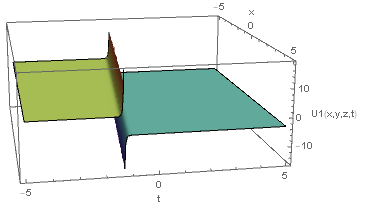
\includegraphics[width=\linewidth,
            height=55mm]{u1.png}\subcaption{} \end{minipage}\qquad\qquad\qquad
            \begin{minipage}{.30\textwidth} 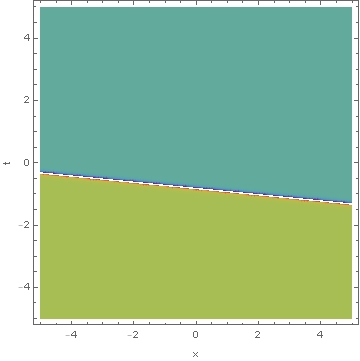
\includegraphics[width=\linewidth,
             height=55mm]{d1.png}\subcaption{} \end{minipage}\\\
              \begin{minipage}{.50\textwidth} 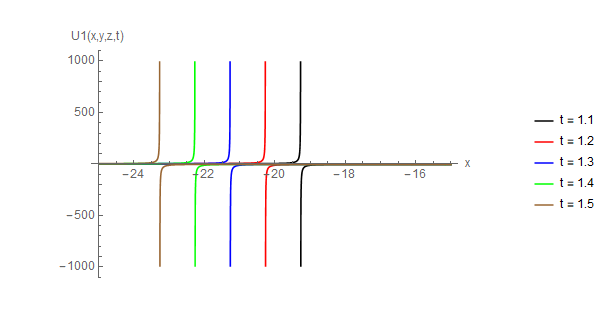
\includegraphics[width=\linewidth,
            height=55mm]{c1.png}\subcaption{} \end{minipage}
    \end{tabular}%
 \noindent\caption {Parameters ${N=-1}$, \,${K=0.021}$, \,${L=397}$, \,${\beta=2}$, \,${\alpha=3}$, \,${v=1.5}$ and \,${\psi=3}$ in \ref{U1} yields the 2D, 3D and density plot of $U_1(\xi)$ which are displayed here.}\label{F1}
\end{figure}\\\
\begin{figure}[h!]
    \centering
    \begin{tabular}{ccc}
        \begin{minipage}{.30\textwidth} 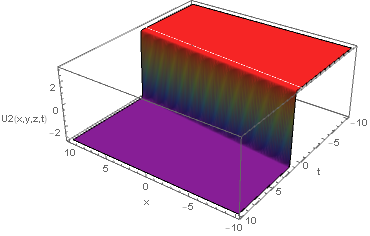
\includegraphics[width=\linewidth,
            height=55mm]{u2.png}\subcaption{} \end{minipage}\qquad\qquad\qquad
            \begin{minipage}{.30\textwidth} 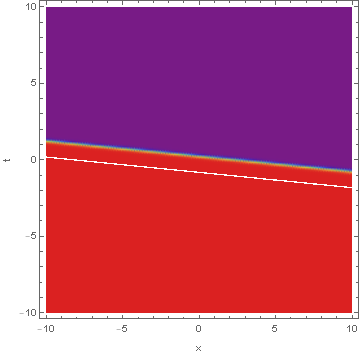
\includegraphics[width=\linewidth,
             height=55mm]{d2.png}\subcaption{} \end{minipage}\\\
              \begin{minipage}{.50\textwidth} 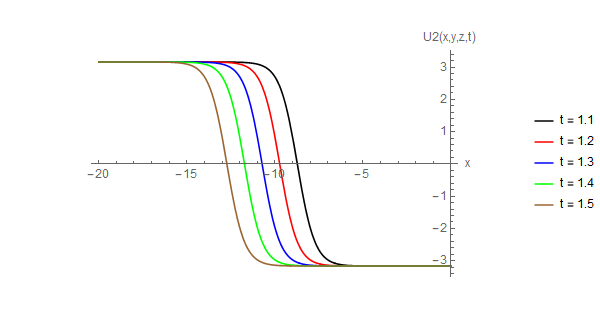
\includegraphics[width=\linewidth,
            height=55mm]{c2.png}\subcaption{} \end{minipage}
    \end{tabular}%
 \noindent\caption{Parameters ${N=-1}$, \,${K=0.021}$, \,${L=397}$, \,${\beta=2}$, \,${\alpha=3}$, \,${v=1.5}$ and \,${\psi=3}$ in \ref{U2} yields the 2D, 3D and density plot of $U_2(\xi)$ which are displayed here.}\label{F2}
\end{figure}\\\
\begin{figure}[h!]
    \centering
    \begin{tabular}{ccc}
        \begin{minipage}{.30\textwidth} 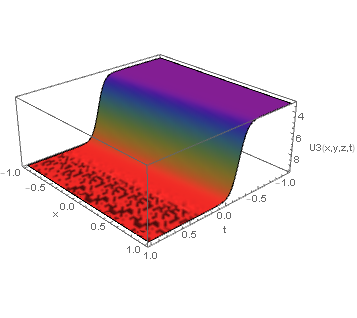
\includegraphics[width=\linewidth,
            height=55mm]{u3.png}\subcaption{} \end{minipage}\qquad\qquad\qquad
            \begin{minipage}{.30\textwidth} 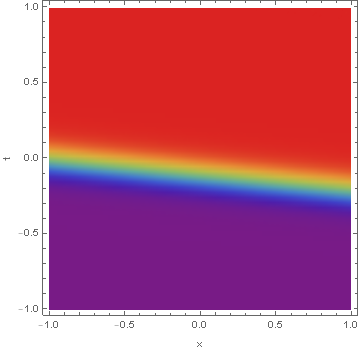
\includegraphics[width=\linewidth,
             height=55mm]{d3.png}\subcaption{} \end{minipage}\\\
              \begin{minipage}{.50\textwidth} 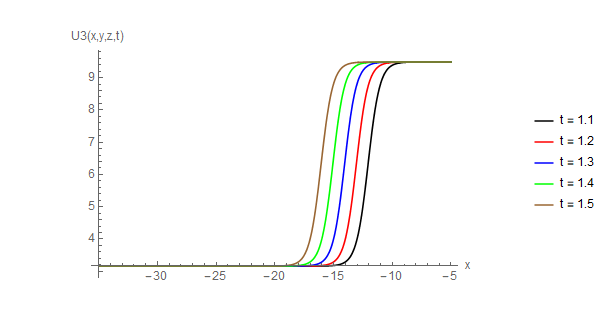
\includegraphics[width=\linewidth,
            height=55mm]{c3.png}\subcaption{} \end{minipage}
    \end{tabular}%
 \noindent\caption{Parameters ${N=-1}$, \,${K=0.021}$, \,${L=397}$, \,${\beta=2}$, \,${\alpha=3}$, \,${v=1.5}$ and \,${\psi=3}$ in \ref{U3} yields the 2D, 3D and density plot of $U_3(\xi)$ which are displayed here.}\label{F3}
\end{figure}\\\
\begin{figure}[h!]
    \centering
    \begin{tabular}{ccc}
        \begin{minipage}{.30\textwidth} 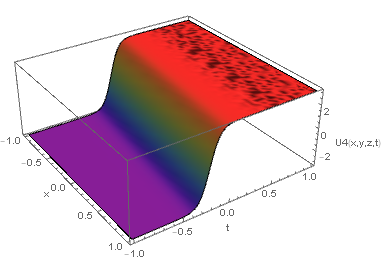
\includegraphics[width=\linewidth,
            height=55mm]{u4.png}\subcaption{} \end{minipage}\qquad\qquad\qquad
            \begin{minipage}{.30\textwidth} 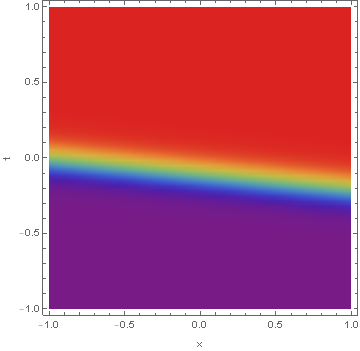
\includegraphics[width=\linewidth,
             height=55mm]{d4.png}\subcaption{} \end{minipage}\\\
              \begin{minipage}{.50\textwidth} 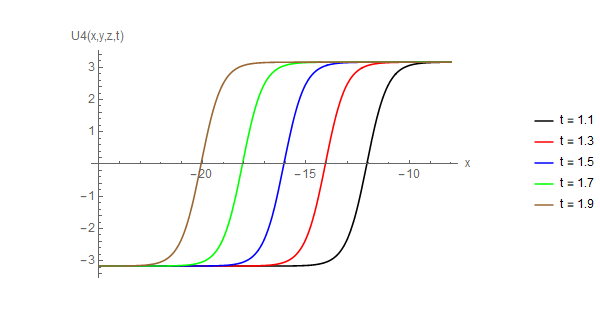
\includegraphics[width=\linewidth,
            height=55mm]{c4.png}\subcaption{} \end{minipage}
    \end{tabular}%
 \noindent\caption{Parameters ${N=-1}$, \,${K=0.021}$, \,${L=397}$, \,${\beta=2}$, \,${\alpha=3}$, \,${v=1.5}$ and \,${\psi=3}$ in \ref{U4} yields the 2D, 3D and density plot of $U_1(\xi)$ which are displayed here.}\label{F4}
\end{figure}\\\
\begin{figure}[h!]
    \centering
    \begin{tabular}{ccc}
        \begin{minipage}{.30\textwidth} 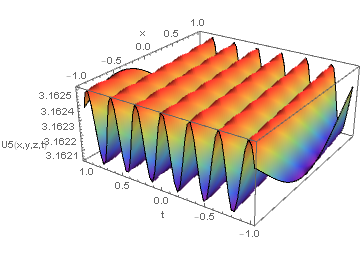
\includegraphics[width=\linewidth,
            height=55mm]{u5.png}\subcaption{} \end{minipage}\qquad\qquad\qquad
            \begin{minipage}{.30\textwidth} 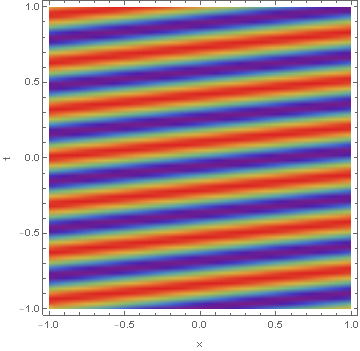
\includegraphics[width=\linewidth,
             height=55mm]{d5.png}\subcaption{} \end{minipage}\\\
              \begin{minipage}{.50\textwidth} 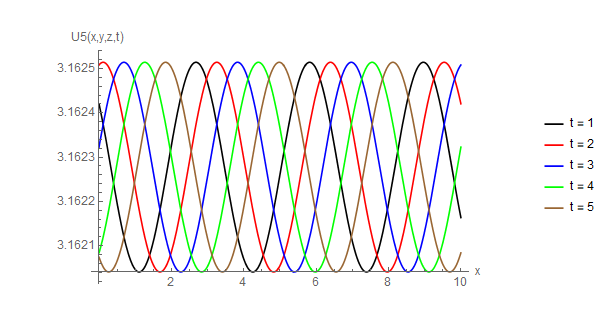
\includegraphics[width=\linewidth,
            height=55mm]{c5.png}\subcaption{} \end{minipage}
    \end{tabular}%
 \noindent\caption{Parameters ${N=1}$, \,${K=0.021}$, \,${L=397}$, \,${\beta=2}$, \,${\alpha=3}$, \,${v=1.5}$ and \,${\psi=3}$ in \ref{U5} yields the 2D, 3D and density plot of $U_5(\xi)$ which are displayed here.}\label{F5}
\end{figure}\\\
\begin{figure}[h!]
    \centering
    \begin{tabular}{ccc}
        \begin{minipage}{.30\textwidth} 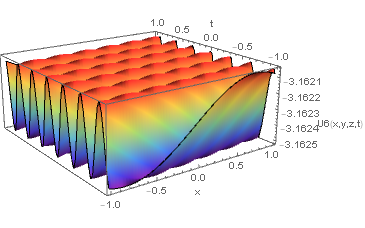
\includegraphics[width=\linewidth,
            height=55mm]{u6.png}\subcaption{} \end{minipage}\qquad\qquad\qquad
            \begin{minipage}{.30\textwidth} 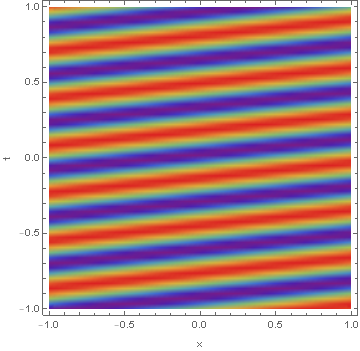
\includegraphics[width=\linewidth,
             height=55mm]{d6.png}\subcaption{} \end{minipage}\\\
              \begin{minipage}{.50\textwidth} 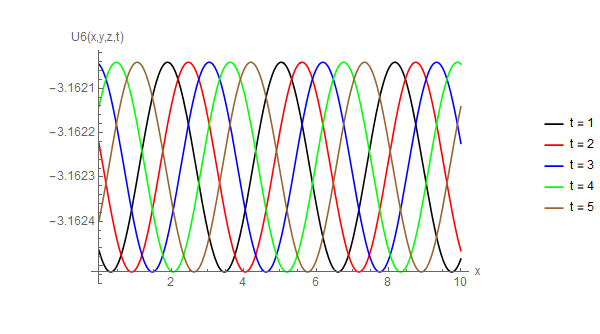
\includegraphics[width=\linewidth,
            height=55mm]{c6.png}\subcaption{} \end{minipage}
    \end{tabular}%
 \noindent\caption{Parameters ${N=1}$, \,${K=0.021}$, \,${L=397}$, \,${\beta=2}$, \,${\alpha=3}$, \,${v=1.5}$ and \,${\psi=3}$ in \ref{U6} yields the 2D, 3D and density plot of $U_6(\xi)$ which are displayed here.}\label{F6}
\end{figure}\\\
\begin{figure}[h!]
    \centering
    \begin{tabular}{ccc}
        \begin{minipage}{.30\textwidth} 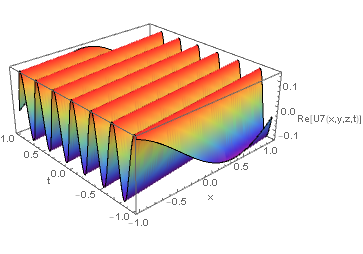
\includegraphics[width=\linewidth,
            height=55mm]{u7r.png}\subcaption{} \end{minipage}\qquad\qquad\qquad
            \begin{minipage}{.30\textwidth} 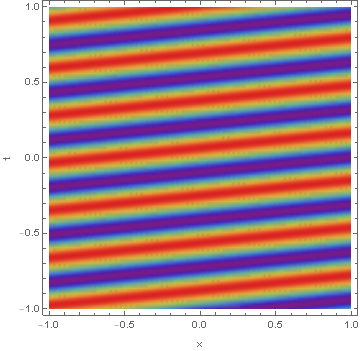
\includegraphics[width=\linewidth,
             height=55mm]{d7r.png}\subcaption{} \end{minipage}\\\
              \begin{minipage}{.50\textwidth} 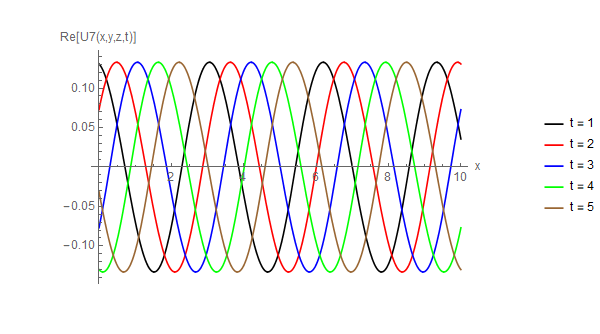
\includegraphics[width=\linewidth,
            height=55mm]{c7r.png}\subcaption{} \end{minipage}
    \end{tabular}%
 \noindent\caption{Parameters ${N=1}$, \,${K=0.021}$, \,${L=397}$, \,${\beta=2}$, \,${\alpha=3}$, \,${v=1.5}$ and \,${\psi=3}$ in \ref{U7} yields the 2D, 3D and density plot of $U_7[Re](\xi)$ which are displayed here.}\label{F7r}
\end{figure}\\\
\begin{figure}[h!]
    \centering
    \begin{tabular}{ccc}
        \begin{minipage}{.30\textwidth} 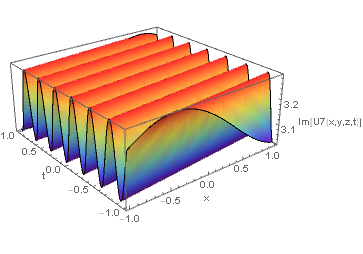
\includegraphics[width=\linewidth,
            height=55mm]{u7i.png}\subcaption{} \end{minipage}\qquad\qquad\qquad
            \begin{minipage}{.30\textwidth} 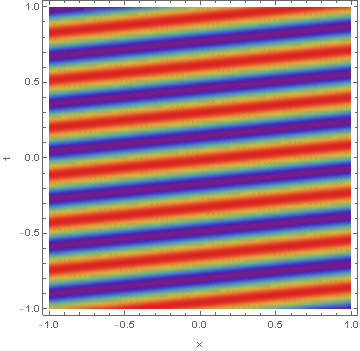
\includegraphics[width=\linewidth,
             height=55mm]{d7i.png}\subcaption{} \end{minipage}\\\
              \begin{minipage}{.50\textwidth} 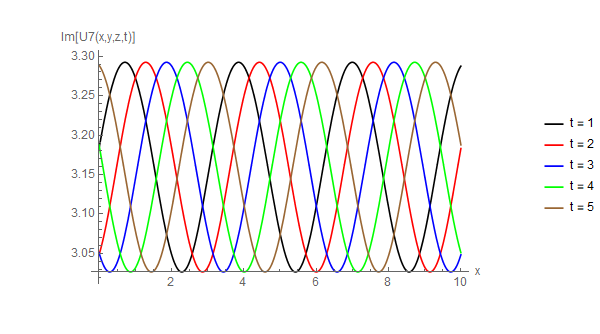
\includegraphics[width=\linewidth,
            height=55mm]{c7i.png}\subcaption{} \end{minipage}
    \end{tabular}%
 \noindent\caption{Parameters ${N=1}$, \,${K=0.021}$, \,${L=397}$, \,${\beta=2}$, \,${\alpha=3}$, \,${v=1.5}$ and \,${\psi=3}$ in \ref{U7} yields the 2D, 3D and density plot of $U_7[Im](\xi)$ which are displayed here.}\label{F7i}
\end{figure}\\\
\begin{figure}[h!]
    \centering
    \begin{tabular}{ccc}
        \begin{minipage}{.30\textwidth} 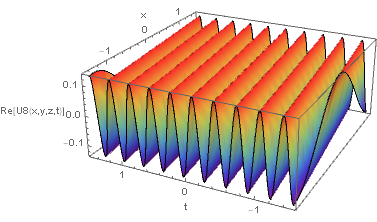
\includegraphics[width=\linewidth,
            height=55mm]{u8r.png}\subcaption{} \end{minipage}\qquad\qquad\qquad
            \begin{minipage}{.30\textwidth} 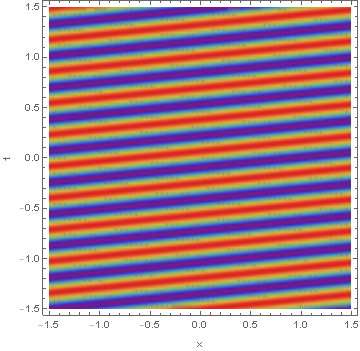
\includegraphics[width=\linewidth,
             height=55mm]{d8r.png}\subcaption{} \end{minipage}\\\
              \begin{minipage}{.50\textwidth} 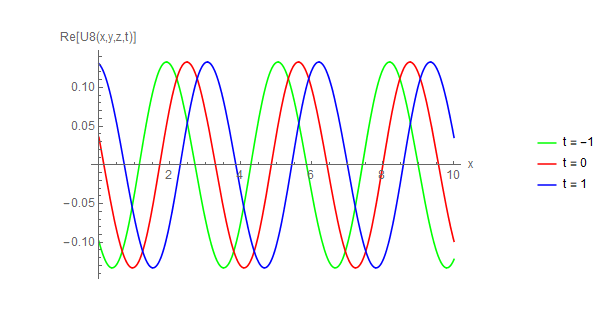
\includegraphics[width=\linewidth,
            height=55mm]{c8r.png}\subcaption{} \end{minipage}
    \end{tabular}%
 \noindent\caption{Parameters ${N=1}$, \,${K=0.021}$, \,${L=397}$, \,${\beta=2}$, \,${\alpha=3}$, \,${v=1.5}$ and \,${\psi=3}$ in \ref{U8} yields the 2D, 3D and density plot of $U_8[Re](\xi)$ which are displayed here.}\label{F8r}
\end{figure}\\\
\begin{figure}[h!]
    \centering
    \begin{tabular}{ccc}
        \begin{minipage}{.30\textwidth} 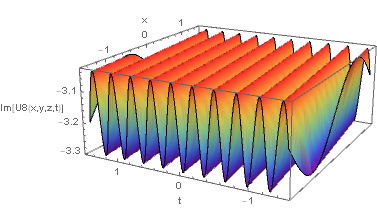
\includegraphics[width=\linewidth,
            height=55mm]{u8i.png}\subcaption{} \end{minipage}\qquad\qquad\qquad
            \begin{minipage}{.30\textwidth} 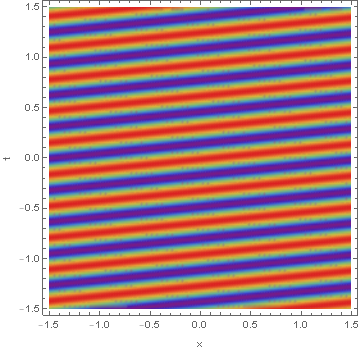
\includegraphics[width=\linewidth,
             height=55mm]{d8i.png}\subcaption{} \end{minipage}\\\
              \begin{minipage}{.50\textwidth} 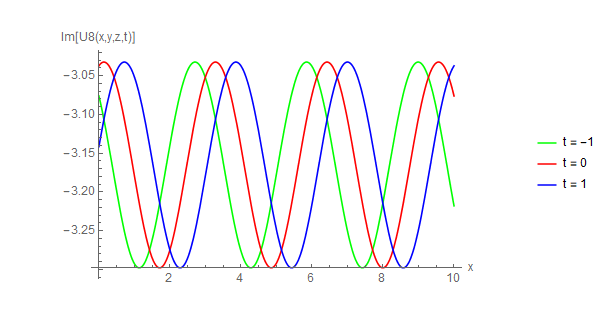
\includegraphics[width=\linewidth,
            height=55mm]{c8i.png}\subcaption{} \end{minipage}
    \end{tabular}%
 \noindent\caption{Parameters ${N=1}$, \,${K=0.021}$, \,${L=397}$, \,${\beta=2}$, \,${\alpha=3}$, \,${v=1.5}$ and \,${\psi=3}$ in \ref{U8} yields the 2D, 3D and density plot of $U_8[Im](\xi)$ which are displayed here.}\label{F8i}
\end{figure}\\\
\begin{figure}[h!]
    \centering
    \begin{tabular}{ccc}
        \begin{minipage}{.30\textwidth} 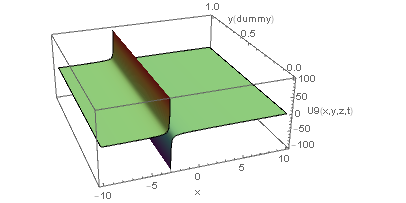
\includegraphics[width=\linewidth,
            height=55mm]{u9.png}\subcaption{} \end{minipage}\qquad\qquad\qquad
            \begin{minipage}{.30\textwidth} 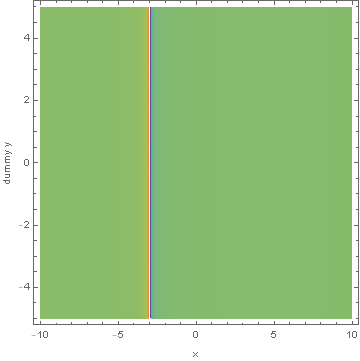
\includegraphics[width=\linewidth,
             height=55mm]{d9.png}\subcaption{} \end{minipage}\\\
              \begin{minipage}{.50\textwidth} 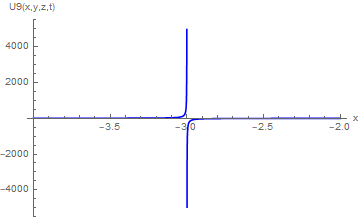
\includegraphics[width=\linewidth,
            height=55mm]{c9.png}\subcaption{} \end{minipage}
    \end{tabular}%
 \noindent\caption{Parameters ${N=0}$, \,${K=0.021}$, \,${L=397}$, \,${\beta=2}$, \,${\alpha=3}$, \,${v=1.5}$ and \,${\psi=3}$ in \ref{U9} yields the 2D, 3D and density plot of $U_9(\xi)$ which are displayed here.}\label{F9}
\end{figure}\\\
\begin{figure}[h!]
    \centering
    \begin{tabular}{ccc}
        \begin{minipage}{.30\textwidth} 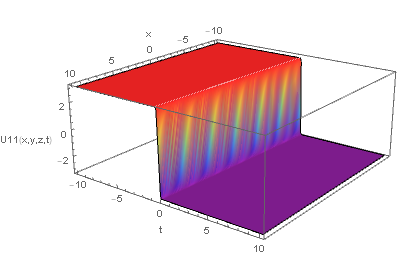
\includegraphics[width=\linewidth,
            height=55mm]{u11.png}\subcaption{} \end{minipage}\qquad\qquad\qquad
            \begin{minipage}{.30\textwidth} 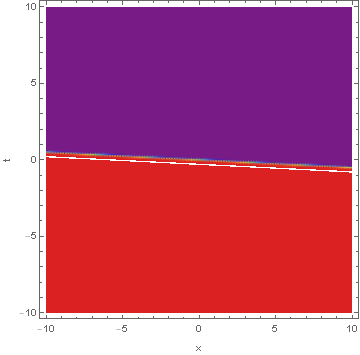
\includegraphics[width=\linewidth,
             height=55mm]{d11.png}\subcaption{} \end{minipage}\\\
              \begin{minipage}{.50\textwidth} 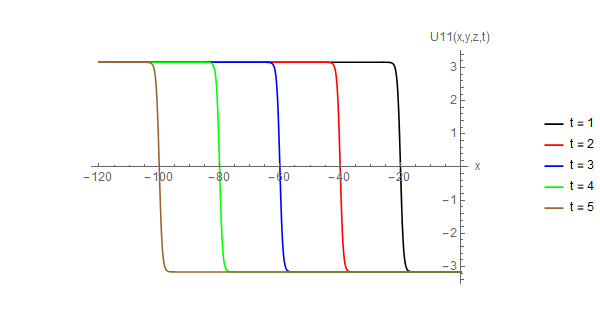
\includegraphics[width=\linewidth,
            height=55mm]{c11.png}\subcaption{} \end{minipage}
    \end{tabular}%
 \noindent\caption{Parameters ${N=-1}$, \,${K=0.021}$, \,${L=4}$, \,${\beta=2}$, \,${\alpha=3}$, \,${v=1.5}$ and \,${\psi=3}$ in \ref{U11} yields the 2D, 3D and density plot of $U_{11}(\xi)$ which are displayed here.}\label{F11}
\end{figure}\\\
\begin{figure}[h!]
    \centering
    \begin{tabular}{ccc}
        \begin{minipage}{.30\textwidth} 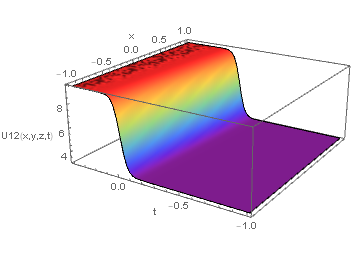
\includegraphics[width=\linewidth,
            height=55mm]{u12.png}\subcaption{} \end{minipage}\qquad\qquad\qquad
            \begin{minipage}{.30\textwidth} 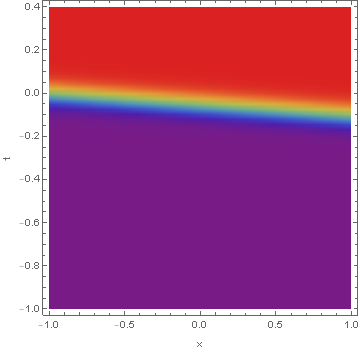
\includegraphics[width=\linewidth,
             height=55mm]{d12.png}\subcaption{} \end{minipage}\\\
              \begin{minipage}{.50\textwidth} 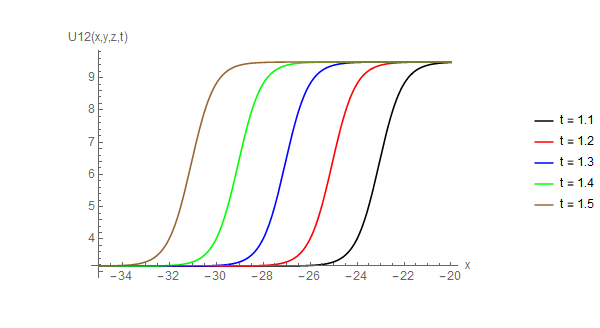
\includegraphics[width=\linewidth,
            height=55mm]{c12.png}\subcaption{} \end{minipage}
    \end{tabular}%
 \noindent\caption{Parameters ${N=-1}$, \,${K=0.021}$, \,${L=4}$, \,${\beta=2}$, \,${\alpha=3}$, \,${v=1.5}$ and \,${\psi=3}$ in \ref{U12} yields the 2D, 3D and density plot of $U_{12}(\xi)$ which are displayed here.}\label{F12}
\end{figure}\\\
\begin{figure}[h!]
    \centering
    \begin{tabular}{ccc}
        \begin{minipage}{.30\textwidth} 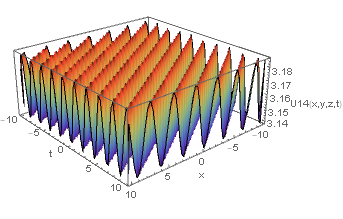
\includegraphics[width=\linewidth,
            height=55mm]{u14.png}\subcaption{} \end{minipage}\qquad\qquad\qquad
            \begin{minipage}{.30\textwidth} 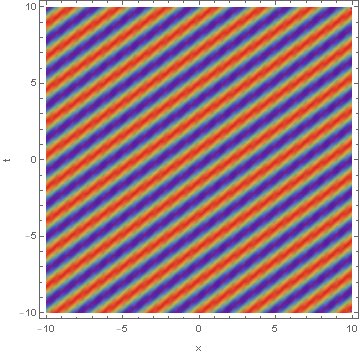
\includegraphics[width=\linewidth,
             height=55mm]{d14.png}\subcaption{} \end{minipage}\\\
              \begin{minipage}{.50\textwidth} 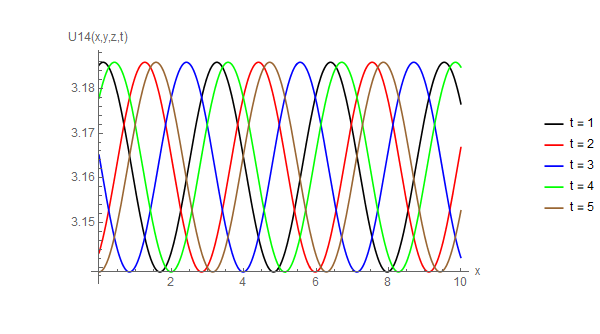
\includegraphics[width=\linewidth,
            height=55mm]{c14.png}\subcaption{} \end{minipage}
    \end{tabular}%
 \noindent\caption{Parameters ${N=1}$, \,${K=0.021}$, \,${L=4}$, \,${\beta=2}$, \,${\alpha=3}$, \,${v=1.5}$ and \,${\psi=3}$ in \ref{U14} yields the 2D, 3D and density plot of $U_{14}(\xi)$ which are displayed here.}\label{F14}
\end{figure}\\\
\begin{figure}[h!]
    \centering
    \begin{tabular}{ccc}
        \begin{minipage}{.30\textwidth} 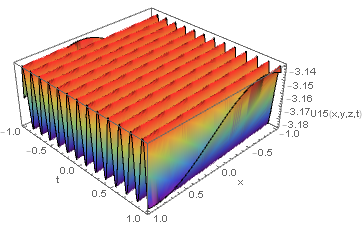
\includegraphics[width=\linewidth,
            height=55mm]{u15.png}\subcaption{} \end{minipage}\qquad\qquad\qquad
            \begin{minipage}{.30\textwidth} 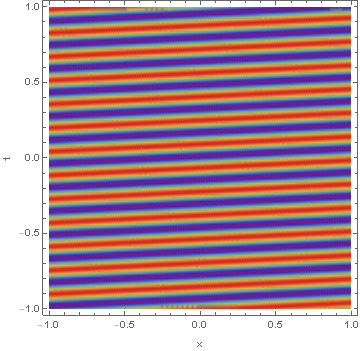
\includegraphics[width=\linewidth,
             height=55mm]{d15.png}\subcaption{} \end{minipage}\\\
              \begin{minipage}{.50\textwidth} 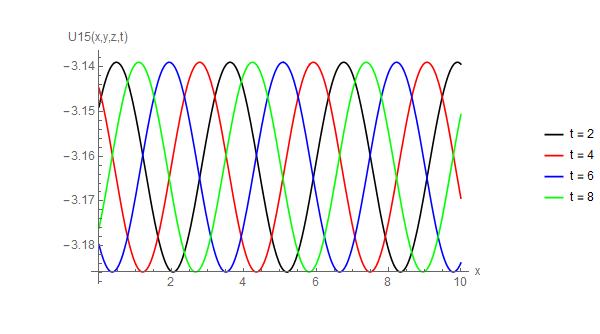
\includegraphics[width=\linewidth,
            height=55mm]{c15.png}\subcaption{} \end{minipage}
    \end{tabular}%
 \noindent\caption{Parameters ${N=1}$, \,${K=0.021}$, \,${L=4}$, \,${\beta=2}$, \,${\alpha=3}$, \,${v=1.5}$ and \,${\psi=3}$ in \ref{U15} yields the 2D, 3D and density plot of $U_{15}(\xi)$ which are displayed here.}\label{F15}
\end{figure}\\\
\begin{figure}[h!]
    \centering
    \begin{tabular}{ccc}
        \begin{minipage}{.30\textwidth} 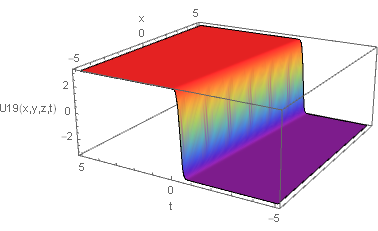
\includegraphics[width=\linewidth,
            height=55mm]{u19.png}\subcaption{} \end{minipage}\qquad\qquad\qquad
            \begin{minipage}{.30\textwidth} 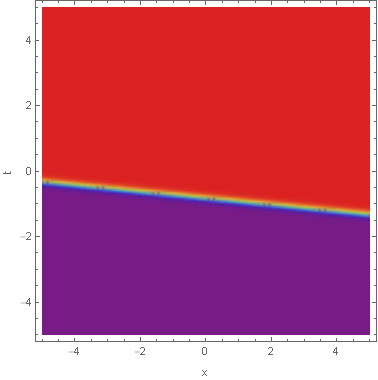
\includegraphics[width=\linewidth,
             height=55mm]{d19.png}\subcaption{} \end{minipage}\\\
              \begin{minipage}{.50\textwidth} 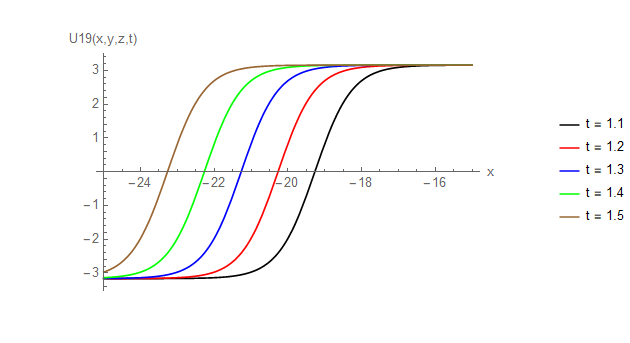
\includegraphics[width=\linewidth,
            height=55mm]{c19.png}\subcaption{} \end{minipage}
    \end{tabular}%
 \noindent\caption{Parameters ${N=-1}$, \,${K=0.021}$, \,${L=397}$, \,${\beta=2}$, \,${\alpha=3}$, \,${v=1.5}$ and \,${\psi=3}$ in \ref{U19} yields the 2D, 3D and density plot of $U_{19}(\xi)$ which are displayed here.}\label{F19}
\end{figure}\\\
\begin{figure}[h!]
    \centering
    \begin{tabular}{ccc}
        \begin{minipage}{.30\textwidth} 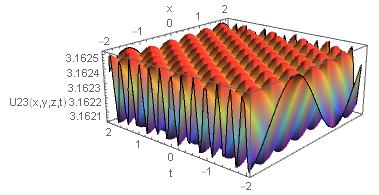
\includegraphics[width=\linewidth,
            height=55mm]{u23.png}\subcaption{} \end{minipage}\qquad\qquad\qquad
            \begin{minipage}{.30\textwidth} 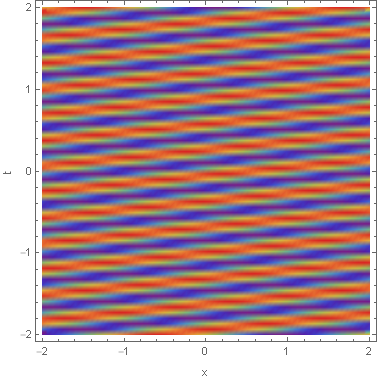
\includegraphics[width=\linewidth,
             height=55mm]{d23.png}\subcaption{} \end{minipage}\\\
              \begin{minipage}{.50\textwidth} 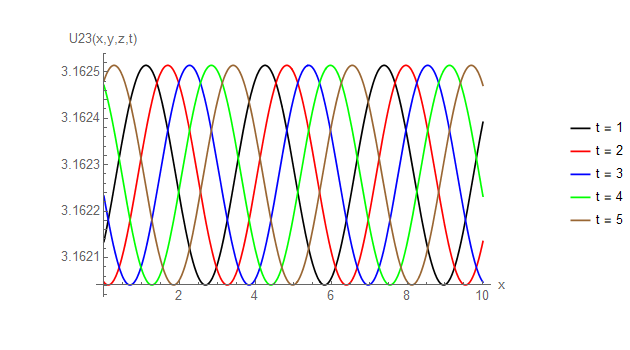
\includegraphics[width=\linewidth,
            height=55mm]{c23.png}\subcaption{} \end{minipage}
    \end{tabular}%
 \noindent\caption{Parameters ${N=1}$, \,${K=0.021}$, \,${L=397}$, \,${\beta=2}$, \,${\alpha=3}$, \,${v=1.5}$ and \,${\psi=3}$ in \ref{U23} yields the 2D, 3D and density plot of $U_{23}(\xi)$ which are displayed here.}\label{F23}
\end{figure}\\\
\begin{figure}[h!]
    \centering
    \begin{tabular}{ccc}
        \begin{minipage}{.30\textwidth} 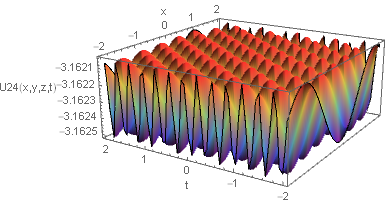
\includegraphics[width=\linewidth,
            height=55mm]{u24.png}\subcaption{} \end{minipage}\qquad\qquad\qquad
            \begin{minipage}{.30\textwidth} 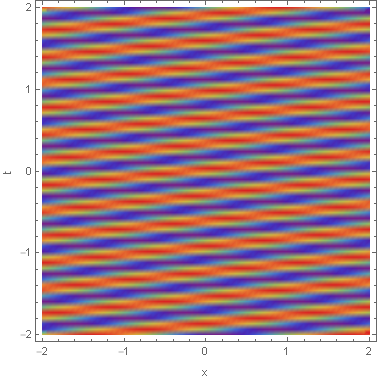
\includegraphics[width=\linewidth,
             height=55mm]{d24.png}\subcaption{} \end{minipage}\\\
              \begin{minipage}{.50\textwidth} 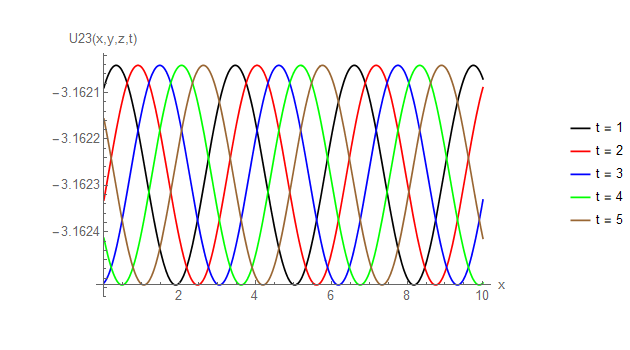
\includegraphics[width=\linewidth,
            height=55mm]{c24.png}\subcaption{} \end{minipage}
    \end{tabular}%
 \noindent\caption{Parameters ${N=-1}$, \,${K=0.021}$, \,${L=397}$, \,${\beta=2}$, \,${\alpha=3}$, \,${v=1.5}$ and \,${\psi=3}$ in \ref{U24} yields the 2D, 3D and density plot of $U_{24}(\xi)$ which are displayed here.}\label{F24}
\end{figure}\\\
\FloatBarrier
\section{Analysis of Bifurcation}
In order to examine all possible phase pictures for the system, the model in question is transformed into a dynamical system via a Galilean transformation in this section. Using Eq. \ref{ODE1} we have
\begin{eqnarray}
 -c\,U+\kappa \frac{U^3}{3}+ (\mu+2\upsilon)U''=0,
\end{eqnarray}
We can write it as
\begin{eqnarray}\label{ODE2}
U^{''}{(\zeta)}=R\,U-S\,U^3,
\end{eqnarray}
where $R=\frac{c}{\mu+2\upsilon}$ and $S= \frac{\kappa}{3(\mu+2\upsilon)}$.\\
It is established from references \cite{b44,b45} that Eq. \ref{ODE2} is comparable to the dynamical system that is linear.\\
\begin{eqnarray}\label{BA}
\frac{d U}{d \zeta} = T,\nonumber
\end{eqnarray}
\begin{eqnarray}
\frac{d T}{d \zeta} = -S \,U^{3}+R U.
\end{eqnarray}
The exact traveling wave solutions for Eq. \ref{PDE1} are defined by the phase trajectories of Eq. \ref{BA} in accordance with the theory of planar dynamical systems. Examine a continuous solution $U(\zeta)$ of Eq. \ref{BA} satisfying ${\lim_{m\longrightarrow-\infty}U(\zeta)=P_{1}}$ and ${\lim_{m\longrightarrow\infty}U(\zeta)=P_{2}}$. Should $P_{1}$ equal $P_{2}$, then $U(\zeta)$ constitutes a homoclinic orbit, and consequently, $u(x,y,z, t)$ is a solitary wave solution. In the case where $P_{1} > P_{2}$,  forms a heteroclinic orbit, resulting in $u(x,y,z, t)$ being a kink wave solution; an antikink wave solution arises for  $P_{1} < P_{2}$. Additionally, a periodic solution of Eq. \ref{PDE1} is represented by each closed curve in the phase portraits of Eq. \ref{BA}. To facilitate this analysis, the Hamiltonian function $H(U, T)$ is sought, defined such that $\frac{\partial H}{\partial T} = \mathit{U'}$  and $\frac{\partial T}{\partial \zeta} = -\mathit{T'}$ . This leads to the system
\begin{eqnarray}
\frac{\partial U}{\partial T} = T,\nonumber
\end{eqnarray}
\begin{eqnarray}
\frac{\partial H}{\partial U} =-T'= -(-S \,U^{3}+R U).
\end{eqnarray}
From Eq. \ref{BA}, it follows that $H(U, T)=\frac{T^2}{2}+f(U)$ where $f(U)$ is an arbitrary function of U. Consequently, $\frac{\partial H(U,T)}{\partial U} =-f'(U)$ and Integrating this yields $f(U)=S\,\frac{U^4}{4}-R\,\frac{U^2}{2}+a_{0}$ with $a_{0}$ as an arbitrary constant. Thus, the Hamiltonian is $H(U, T) = \frac{T^2}{2}+S\,\frac{U^4}{4}-R\,\frac{U^2}{2}+a_{0}$. By selecting the constant appropriately, one obtains\\
\begin{eqnarray}
H(U, V) = \frac{T^2}{2}+S\,\frac{U^4}{4}-R\,\frac{U^2}{2}=a_{1},
\end{eqnarray}
here, $T$ denotes the generalized momentum, $U$ the generalized coordinate, $\frac{T^2}{2}$ the kinetic energy, and $\,\frac{U^4}{4}-R\,\frac{U^2}{2}$ the potential energy, with $h_{1}$ representing the total energy constant.\\
The equilibrium points $E(U, T)$ for Eq. \ref{BA} are found by solving the system derived from setting $\frac{d U}{d \zeta}= 0$ and $\frac{d T}{d \zeta} = 0$
\begin{eqnarray}\label{EP}
0 = T,\nonumber
\end{eqnarray}
\begin{eqnarray}
0 = -S \,U^{3}+R U.
\end{eqnarray}
By using Eq. \ref{EP} obtain solutions for $U$. The first equation gives $T = 0$. The second equation yields $U=0$, $U=\sqrt{\frac{R}{S}}$ and $U=-\sqrt{\frac{R}{S}}$. Therefore, if $RS < 0$, the sole equilibrium point is $E_{1}(0, 0)$. If $RS > 0$, there exist three equilibrium points: $E_{1}(0, 0), E_{2}(\sqrt{\frac{R}{S}},0)$ and $E_{3}(-\sqrt{\frac{R}{S}}, 0)$.\\
The Jacobian matrix $J(U, T)$ for the Hamiltonian system at an equilibrium point $(U_{0},T_{0})$ is given by
\begin{eqnarray}
\frac{d U}{d \zeta} = \frac{\partial H}{\partial T},
\end{eqnarray}
\begin{eqnarray}
\frac{d T}{d \zeta} = -\frac{\partial H}{\partial U},
\end{eqnarray}
\begin{equation}
J(U, V) =
\begin{bmatrix}
\dfrac{\partial^2 H}{\partial U \, \partial T} & \dfrac{\partial^2 H}{\partial T^2} \\[8pt]
-\dfrac{\partial^2 H}{\partial U^2} & -\dfrac{\partial^2 H}{\partial T \, \partial U}
\end{bmatrix}_{(U_0, T_0)},
\end{equation}
For the specific system Eq. \ref{BA}, this evaluates to\\
\begin{center}
$J(U, V) =
\begin{bmatrix}
 0 & 1 \\[8pt]
 R-3\,S\,U^2 & 0
\end{bmatrix},$
\end{center}
with its determinant being
\begin{center}
$ |J (U, T)| = -(R-3\,S\,U^2).$
\end{center}
Here are the bifurcations of the system's phase portraits.\\
\begin{figure}[h!]
    \centering
    \begin{tabular}{ccc}
        \begin{minipage}{.30\textwidth} 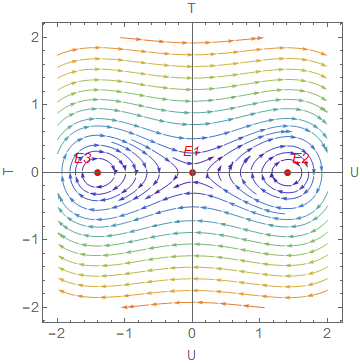
\includegraphics[width=\linewidth,
            height=55mm]{p1.png}\subcaption{} \end{minipage}
    \end{tabular}%
 \noindent\caption{The phase portrait bifurcation of Eq. \ref{BA} for $R>0$ and $S>0$. }\label{B1}
\end{figure}\\
\begin{figure}[h!]
    \centering
    \begin{tabular}{ccc}
        \begin{minipage}{.30\textwidth} 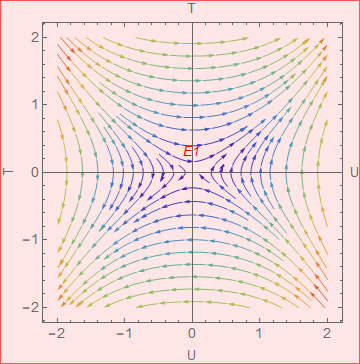
\includegraphics[width=\linewidth,
            height=55mm]{p2.png}\subcaption{} \end{minipage}
    \end{tabular}%
 \noindent\caption{The phase portrait bifurcation of Eq. \ref{BA} for $R>0$ and $S<0$.}\label{B2}
\end{figure}\\
\begin{figure}[h!]
    \centering
    \begin{tabular}{ccc}
        \begin{minipage}{.30\textwidth} 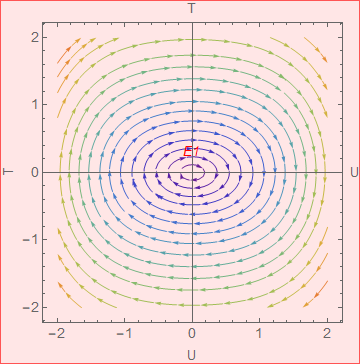
\includegraphics[width=\linewidth,
            height=55mm]{p3.png}\subcaption{} \end{minipage}
    \end{tabular}%
 \noindent\caption{The phase portrait bifurcation of Eq. \ref{BA} for $R<0$ and $S>0$.}\label{B3}
\end{figure}\\
\begin{figure}[h!]
    \centering
    \begin{tabular}{ccc}
        \begin{minipage}{.30\textwidth} 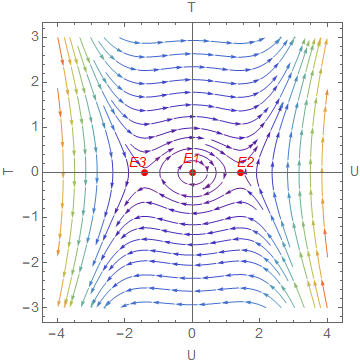
\includegraphics[width=\linewidth,
            height=55mm]{p4.png}\subcaption{} \end{minipage}
    \end{tabular}%
 \noindent\caption{The phase portrait bifurcation of Eq. \ref{BA} for $R<0$ and $S<0$.}\label{B4}
\end{figure}
\noindent
\newpage
The categorization provided by the bifurcation theory for planar dynamical systems is as follows:\\
\textbf{Theorem:} For an equilibrium point $E(U_{0}, T_{0})$, if $|J(E)| < 0$, it is a saddle point, if $|J(E)| > 0$ and the $Trace(J(E)) = 0$, it is a center point and if $|J(E)| = 0$, $Trace(J(E)) = 0$, and its Poincare index is $0$, it is a cusp point.\\
Based on this, the bifurcation analysis for different parameter ranges is as follows:\\
\textbf{Preposition:}
\begin{itemize}
  \item \textbf{For $R > 0$, $S > 0$:} The system possesses three equilibrium points $E_{1}(0, 0), E_{2}(\sqrt{\frac{R}{S}},0)$ and $E_{3}(-\sqrt{\frac{R}{S}}, 0)$. The origin $E_{1}(0, 0)$ is a saddle point as $|J(E_{1})| < 0$ and a homoclinic orbit originates from and returns to the point $E_{1}(0, 0)$. The points $E_{2}(\sqrt{\frac{R}{S}},0)$ and $E_{3}(-\sqrt{\frac{R}{S}}, 0)$ are centers because $|J(E_{2,3})| > 0$ and $Trace(E_{2,3})=0$ each surrounded by a family of periodic orbits. The phase portrait of it is displayed in Fig. (\ref{B1}).
  \item \textbf{For $R> 0$, $S < 0$:} The only equilibrium point is $E_{1}(0, 0)$. This point is a saddle point $|J(E_{1})| < 0$. Consequently, no closed trajectories exist, meaning Eq. \ref{BA} has no periodic solutions. The phase portrait for different parameters is depicted in Fig. (\ref{B2}).
  \item \textbf{For $R < 0$, $S < 0$:} The system possesses three equilibrium points $E_{1}(0, 0), E_{2}(\sqrt{\frac{R}{S}},0)$ and $E_{3}(-\sqrt{\frac{R}{S}}, 0)$. The origin $E_{1}(0, 0)$ is a centre point as $|J(E_{1})| > 0$ and $Trace(E_{1})=0$ giving rise to a family of periodic orbits around it which correspond to periodic wave solutions for Eq. \ref{ODE2}. The points $E_{2}$ and $E_{3}$ are saddle points $|J(E_{2,3})| < 0$. The heteroclinic orbits connecting these saddles indicate the existence of solitary wave solutions. Fig. (\ref{B3}) shows a sample phase picture for arbitrary values. A homoclinic orbit originates from and returns to the point $E_{1}(0, 0)$. The points $E_{2}(\sqrt{\frac{R}{S}},0)$ and $E_{3}(-\sqrt{\frac{R}{S}}, 0)$ are centers because $|J(E_{2,3})| > 0$ and $Trace(E_{2,3})=0$ each surrounded by a family of periodic orbits. The phase portrait of it is displayed in Fig. (\ref{B3}).
  \item \textbf{For $R < 0$, $S > 0$:} The only equilibrium point is $E_{1}(0, 0)$. This point is a center $|J(E_{1})| > 0$, $Trace=0$). All surrounding orbits are closed curves, indicating that Eq. \ref{ODE2} admits solely periodic solutions. Fig. (\ref{B4}) displays the equivalent phase picture with arbitrary settings..
\end{itemize}
\section{Results and Discussion}\label{s4}
\noindent
The (3+1)-dimensional KdV-ZK problem has produced several families of accurate traveling-wave solutions when the unified approach method is applied. These solutions are stated in terms of rational, trigonometric and hyperbolic functions. These solutions are categorized into three distinct sets based on the parameters obtained from the balancing procedure and auxiliary Riccati equation.\\
\begin{itemize}
  \item \textbf{Set I} corresponds to the case where $F_{1}=0$, leading to solutions that include bright/dark soliton profiles for $N<0$ and periodic wave patterns for $N>0$.
  \item \textbf{Set II} and \textbf{Set III} incorporate non-zero $F_{1}$ and exhibit combined soliton structures, including singular periodic waves and complex-valued wave profiles.
  \item Graphical simulations confirm the physical realism of these solutions, showcasing wave propagation, amplitude variation, and localization features in 2D, 3D and density plots.
\end{itemize}

The bifurcation analysis of the equivalent planar Hamiltonian system reveals that the nature of solutions is governed by the signs of parameters A and B:
\begin{itemize}
  \item For $R>0$,$S>0$, The system supports both periodic and homoclinic orbits (solitary waves) and admits three equilibrium points: a saddle at the origin and two centers.
  \item For $R>0$,$S<0$, only a saddle point exists, precluding periodic solutions.
  \item For $R<0$,$S>0$, a single center gives rise exclusively to periodic waves.
  \item For $R<0$,$S<0$, two saddle points connected by heteroclinic orbits indicate kink/antikink solutions whereas periodic orbits round the origin, which turns into a center.
\end{itemize}
These phase portraits provide a complete qualitative description of all possible wave patterns supported by the model, linking analytical solutions directly to dynamical systems theory.
\section{Conclusion}\label{s5}
\noindent In this work, a mixed analytical and dynamical approach is used to explore the (3+1)-dimensional KdV-ZK problem. The available solution set of the model is greatly increased by using the unified technique, which is demonstrated to be an effective tool for generating a wide class of accurate soliton solutions, including kink-type, singular and periodic waves. The simplified dynamical system's basic phase-space structure is revealed by complementary bifurcation analysis, which makes it possible to categorize wave behaviors according to equilibrium stability and parameter variations. This combined method offers a dynamical explanation for the development of wave solutions in addition to precise formulations for them. The results have applications in fluid dynamics, nonlinear optics and plasma physics, where localized wave phenomena are crucial. In addition to applying the concept to additional higher-dimensional non-linear evolution equations, further research may concentrate on symmetry reductions, conservation laws and stability characteristics of the found solutions.
\begin{thebibliography}{99}
\bibitem{b1} Wang, M., Tian, B., Hu, C.-C., ${\&}$ Liu, S.-H. (2021). Generalized Darboux transformation, solitonic interactions and bound states for a coupled fourth-order non-linear Schr\"{o}dinger system in a birefringent optical fiber. \emph{Applied Mathematics Letters, 119}, 106936.
\bibitem{b2} Shen, Y., ${\&}$ Tian, B. (2021). Bilinear auto-B\"{a}cklund transformations and soliton solutions of a (3+1)-dimensional generalized non-linear evolution equation for the shallow water waves. \emph{Applied Mathematics Letters, 122}, 107510.
\bibitem{b3} Gao, X.-T., Tian, B., Shen, Y., ${\&}$ Feng, C.-H. (2021). Comment on: Shallow water in an open sea or a wide channel: Auto and non-auto-B\"{a}cklund transformations with solitons for a generalized dimensional dispersive long-wave system. \emph{Chaos, Solitons {\&} Fractals, 151}, 111222.
\bibitem{b4} Yang, D.-Y., Tian, B., Qu, Q.-X., Zhang, C.-R., Chen, S.-S., et al. (2021). Lax pair, conservation laws, Darboux transformation and localized waves of a variable-coefficient coupled Hirota system in an inhomogeneous optical fiber. \emph{Chaos, Solitons ${\&}$ Fractals, 150}, 110487.
\bibitem{b5} Gao, X.-Y., Guo, Y.-J., ${\&}$ Shan, W.-R. (2021). Optical waves/modes in a multicomponent inhomogeneous optical fiber via a three-coupled variable-coefficient non-linear Schr\"{o}dinger system. \emph{Applied Mathematics Letters, 120}, 107161.
\bibitem{b6}Gao, X.-Y., Guo, Y.-J., ${\&}$ Shan, W.-R. (2021). Beholding the shallow water waves near an ocean beach or in a lake via a Boussinesq-Burgers system. \emph{Chaos, Solitons ${\&}$ Fractals, 147}, 110875.
\bibitem{b7} Cevikel, A.C., ${\&}$ Aksoy, E. (2021). Soliton solutions of non-linear fractional differential equations with their applications in mathematical physics. \emph{Revista Mexicana de Física, 67}, 3.
\bibitem{b8} Cevikel, A.C. (2018). New exact solutions of the space-time fractional KdV-Burgers and non-linear fractional foam drainage equation. \emph{Thermal Science, 22}(1), 15-24.
\bibitem{b9} Aksoy, E., Bekir, A., ${\&}$ Cevikel, A.C. (2019). Study on fractional differential equations with modified Riemann-Liouville derivative via Kudryashov method. \emph{International Journal of Non-linear Sciences and Numerical Simulation, 20}(5), 511-516.
\bibitem{b10} Bekir, A., Guner, O., ${\&}$ Cevikel, A.C. (2017). The exp-function method for some time-fractional differential equations. \emph{IEEE/CAA Journal of Automatica Sinica, 4}(2), 315-321.
\bibitem{b11} Guner, O., Bekir, A., ${\&}$ Cevikel, A.C. (2013). Dark soliton and periodic wave solutions of non-linear evolution equations. \emph{Advances in Difference Equations,} 68.
\bibitem{b12} Cevikel, A.C., Bekir, A., San, S., ${\&}$ Gucen, M.B. (2014). Construction of periodic and solitary wave solutions for the complex non-linear evolution equations. \emph{Journal of the Franklin Institute, 351}(2), 694-700.
\bibitem{b13} Wazwaz, A.M. (2005). Exact solutions to the double sinh-Gordon equation by the tanh method and a variable separated ODE method. \emph{Computers ${\&}$ Mathematics with Applications, 50}(10–12), 1685-1696.
\bibitem{b14} \"{O}zkan, Y.S., Seadawy, A.R., ${\&}$ Yasar, E. (2021). Multi-wave, breather and interaction solutions to (3+1)-dimensional Vakhnenko-Parkes equation arising at propagation of high-frequency waves in a relaxing medium. \emph{Journal of Taibah University for Science, 15}(1), 666-678.
\bibitem{b15} Yang, X.-F., Deng, Z.-C., ${\&}$ Wei, Y. (2015). A Riccati-Bernoulli sub-ODE method for non-linear partial differential equations and its application. \emph{Advances in Difference Equations,} 117.
\bibitem{b16} Ali, L., et al. (2016). New version of optimal homotopy asymptotic method for the solution of non-linear boundary value problems in finite and infinite intervals. \emph{Alexandria Engineering Journal, 55}(3), 2811-2819.
\bibitem{b17} Ali, L., et al. (2018). A new analytical approach for solving non-linear boundary value problems arising in non-linear phenomena.\emph{ Filomat, 32}(7), 2489-2497.
\bibitem{b18} Ali, J., et al. (2012). The optimal homotopy asymptotic method for the solution of higher-order boundary value problems in finite domains. \emph{Abstract and Applied Analysis,} 1-14.
\bibitem{b19} Ali, L., et al. (2017). Magnetohydrodynamics thin film fluid flow under the effect of thermophoresis and variable fluid properties. \emph{AIChE Journal, 63}(12), 5149-5158.
\bibitem{b20} Anil Sezer, S., Yildirim, A., ${\&}$ Tauseef Mohyud-Din, S. (2011). He's homotopy perturbation method for solving the fractional KdV-Burgers-Kuramoto equation. \emph{International Journal of Numerical Methods for Heat and Fluid Flow, 21}(4), 448-458.
\bibitem{b21} Tauseef Mohyud-Din, S., Aslam Noor, M., Noor, K.I., ${\&}$ Hosseini, M.M. (2010). Variational iteration method for re-formulated partial differential equations. \emph{ International Journal of Non-linear Sciences and Numerical Simulation, 11}(2), 87-92.
\bibitem{b22} Shakeel, M., ${\&}$ Mohyud-Din, S.T. (2015). Improved ($\frac{G'}{G}$)-expansion and extended tanh methods for (2+ 1)-dimensional Calogero-Bogoyavlenskii-Schiff equation. \emph{Alexandria Engineering Journal, 54}(1), 27-33.
\bibitem{b23} Guner, O., Atik, H., ${\&}$ Kayyrzhanovich, A.A. (2017). New exact solution for space-time fractional differential equations via ($\frac{G'}{G}$)-expansion method. \emph{Optik-Internatinal Journal for Light and Electron Optics, 130}, 696-701.
\bibitem{b24} Ekici, M. (2017). Soliton and other solutions of non-linear time fractional parabolic equations using extended ($\frac{G'}{G}$)-expansion method. \emph{Optik, 130}, 1312-1319.
\bibitem{b25} Guner, O., Bekir, A., ${\&}$ Bilgil, H. (2015). A note on exp-function method combined with complex transform method applied to fractional differential equations. \emph{Advances in Non-linear Analysis, 4}(3), 201-208.
\bibitem{b26} Navickas, Z., Telksnys, T., ${\&}$ Ragulskis, M. (2015). Comments on ``the exp-function method and generalized solitary solutions". \emph{Computers and Mathematics with Applications, 69}(8), 798-803.
\bibitem{b27} Noor, M.A., Mohyud-Din, S.T., ${\&}$ Waheed, A. (2009). Exp-function method for solving Kuramoto-Sivashinsky and Boussinesq equations. \emph{Journal of Applied Mathematics and Computing, 29}, 1-13.
\bibitem{b28} Mohyud-Din, S.T., Noor, M. A., ${\&}$ Waheed, A. (2009). Exp-function method for generalized traveling solutions of good Boussinesq equations. \emph{Journal of Applied Mathematics and Computing, 30}, 439-445.
\bibitem{b29} Younis, M., ${\&}$ Zafar, A. (2013). The modified simple equation method for solving non-linear Phi-Four equation. \emph{International Journal of Innovation and Applied Studies, 2}(4), 661-664.
\bibitem{b30} Zayed, E.M. (2011). A note on the modified simple equation method applied to Sharma-Tasso-Olver equation. \emph{Applied Mathematics and Computation, 218}(7), 3962-3964.
\bibitem{b31} El-Wakil, S.A., ${\&}$ Abdou, M.A. (2007). New exact travelling wave solutions using modified extended tanh-function method. \emph{Chaos, Solitons and Fractals, 31}(4), 840-852.
\bibitem{b32} Xu, T., Li, J., Zhang, H.Q., Zhang, Y. X., Yao, Z. Z., ${\&}$ Tian, B. (2007). New extension of the tanh-function method and application to the Whitham-Broer-Kaup shallow water model with symbolic computation. \emph{Physics Letters A, 369}(5-6), 458-463.
\bibitem{b33} Inc, M., ${\&}$ Fan, E.G. (2005). Extended tanh-function method for finding travelling wave solutions of some non-linear partial differential equations. \emph{Zeitschrift f\"{u}r Naturforschung A, 60}(1-2), 7-16.
\bibitem{b34} Hosseini, K., Bekir, A., ${\&}$ Ansari, R. (2017). New exact solutions of the conformable time-fractional Cahn-Allen and Cahn-Hilliard equations using the modified Kudryashov method. \emph{Optik, 132}, 203-209.
\bibitem{b35} Kaplan, M., Bekir, A., ${\&}$ Akbulut, A. (2016). A generalized Kudryashov method to some non-linear evolution equations in mathematical physics. \emph{Non-linear Dynamics, 85}, 2843-2850.
\bibitem{b36}Gurefe, Y., Misirli, E., Sonmezoglu, A., ${\&}$ Ekici, M. (2013). Extended trial equation method to generalized non-linear partial differential equations. \emph{Applied Mathematics and Computation, 219}(10), 5253-5260.
\bibitem{b37} Ghosh, S., ${\&}$ Nandy, S. (1999). Inverse scattering method and vector higher order non-linear Schr\"{o}dinger equation. \emph{Nuclear Physics B, 561}(3), 451-466.
\bibitem{b38} Ma, W.X., ${\&}$ Abdeljabbar, A. (2012). A bilinear Bäcklund transformation of a (3+ 1)-dimensional generalized KP equation. \emph{Applied Mathematics Letters, 25}(10), 1500-1504.
\bibitem{b39} Wazwaz, A.M. (2008). The Hirota’s bilinear method and the tanh-coth method for multiple-soliton solutions of the Sawada-Kotera-Kadomtsev-Petviashvili equation. \emph{Applied Mathematics and Computation, 200}(1), 160-166.
\bibitem{b40} Wang, M., Zhou, Y., ${\&}$ Li, Z. (1996). Application of a homogeneous balance method to exact solutions of non-linear equations in mathematical physics. \emph{Physics Letters A, 216}(1-5), 67-75..
\bibitem{b41} Liu, S., Fu, Z., Liu, S., ${\&}$ Zhao, Q. (2001). Jacobi elliptic function expansion method and periodic wave solutions of non-linear wave equations. \emph{Physics Letters A, 289}(1-2), 69-74.
\bibitem{b42} Raza, N., Seadawy, A.R., Kaplan, M., ${\&}$ Butt, A.R. (2021). Symbolic computation and sensitivity analysis of non-linear Kudryashov's dynamical equation with applications. \emph{Physica Scripta, 96}(10), 105216.
\bibitem{b43} Khalique, C. M., ${\&}$ Adeyemo, O.D. (2020). A study of (3+1)-dimensional generalized Korteweg-de Vries-Zakharov-Kuznetsov equation via Lie symmetry approach. \emph{Results in Physics, 20}, 103743.
\bibitem{b44} Li, J., ${\&}$ Liu, Z. (2002). Traveling wave solutions for a class of non-linear dispersive equations. \emph{Chinese Annals of Mathematics, Series B, 23}(3), 397418.
\bibitem{b45} Liang, J., Tang, L., Xia, Y., ${\&}$ Zhang, Y. (2020). Bifurcations and exact solutions for a class of MKdV equations with the conformable fractional derivative via dynamical system method. \emph{International Journal of Bifurcation and Chaos, 30}(1), 2050004
\end{thebibliography}
\end{document}  